\documentclass[french,a4paper,12pt]{report}
\title{Dependency discoverer}
\author{Théophane BOUÉ}
\date{juin 2021}

\usepackage{tabularx}
\usepackage[table]{xcolor}

\usepackage[french]{babel} %french
\usepackage[head=0.5in,includeheadfoot,headsep=.5in,left=1in,right=1in,top=.1in,bottom=0.5in,footskip=0.5in]{geometry} %geometry for margins
\usepackage{eso-pic,graphicx} %eso-pic for background on first page and logos in header
\usepackage{hyperref} %hyperref
%\hypersetup{
%    colorlinks,
%    linkcolor={red!30!black},
%    citecolor={blue!50!black},
%    urlcolor={blue!80!black}
%}

\usepackage{fontspec} %sets custom font
\setmainfont{SourceSansPro}[ 
Path=./ressources/fonts/,
Extension = .ttf,
UprightFont = *-Regular,
ItalicFont  = *-Italic ,
BoldItalicFont = *-BoldItalic,
BoldFont= *-Bold]




\newcommand\AtPageUpperRight[1]{\AtPageUpperLeft{%
   \makebox[.95\paperwidth][r]{#1}}}

 \newcommand\BackgroundLogos{
           \AtPageUpperRight{\raisebox{-\height}{
\includegraphics[width=8cm]{ressources/images/Header-logo.png}}}}



\usepackage{fancyhdr}

\pagestyle{fancy}%
\renewcommand{\chaptermark}[1]{%
\markboth{#1}{}}
\fancyhf{}%
\lhead{ \fontsize{14}{17} \textit{ \textcolor{gray} \leftmark}}%
\cfoot{\thepage}%


\renewcommand{\headrulewidth}{0pt}


\usepackage[toc,page]{appendix}

\hypersetup{
    colorlinks=true,
    linkcolor=blue,
    filecolor=magenta,      
    urlcolor=cyan,
}
\usepackage{listings}
\lstset{language=Java}

\definecolor{codegreen}{rgb}{0,0.6,0}
\definecolor{codegray}{rgb}{0.5,0.5,0.5}
\definecolor{codepurple}{rgb}{0.58,0,0.82}
\definecolor{backcolour}{rgb}{0.95,0.95,0.92}

\lstdefinestyle{javaStyle}{
    %backgroundcolor=\color{backcolour},   
    commentstyle=\color{codegreen},
    keywordstyle=\color{codepurple},
    numberstyle=\tiny\color{codegray},
    stringstyle=\color{blue},
    basicstyle=\ttfamily\footnotesize,
    breakatwhitespace=false,         
    breaklines=true,                 
    captionpos=b,                    
    keepspaces=true,                 
    numbers=left,                    
    numbersep=5pt,                  
    showspaces=false,                
    showstringspaces=false,
    showtabs=false,                  
    tabsize=2
}

\lstset{style=javaStyle}

%%%%%%%%%%%%%%%%%%%%%%%%%%%%%%%%%%%%%%%%%%%%%%%%%%%%%%%%%%%%%%%%%%%%%%%%%%%%%%%%%%%%%%%%%%%%%%%%%%%%%
%%%%%%%%%%%%%%%%%%%%%%%%%%%%%%%%%%%%%%%%BEGINNING%%%%%%%%%%%%%%%%%%%%%%%%%%%%%%%%%%%%%%%%%%%%%%%%%%%%
%%%%%%%%%%%%%%%%%%%%%%%%%%%%%%%%%%%%%%%%%%%%%%%%%%%%%%%%%%%%%%%%%%%%%%%%%%%%%%%%%%%%%%%%%%%%%%%%%%%%%

\begin{document}


\pagestyle{empty}

\pagenumbering{roman} 
\renewcommand{\thepage}{Couverture}

\AddToShipoutPictureBG*{%
{
\includegraphics[width=\paperwidth,height=\paperheight]{ressources/images/premiere4.png}
}}
\null\newpage
\pagenumbering{arabic} 
\pagestyle{plain}

\addcontentsline{toc}{chapter}{Table des matières}
\tableofcontents
\newpage

\pagestyle{fancy}



\chapter*{Lexicon}
\addcontentsline{toc}{chapter}{Lexicon}

\AddToShipoutPicture{\BackgroundLogos}

\hypertarget{API}{\noindent\textbf{API \emph{Application Programming Interface}} interface numérique, permet de donner l'accès à un service.}

\bigskip

\hypertarget{CLI}{\noindent\textbf{CLI} ou interface en lignes de commandes, interface d'un programme permettant une interaction dans un terminal de commandes, donne des informations sur le programme et permet son exécution avec les paramètres donnés. }

\bigskip

\hypertarget{CI}{\noindent\textbf{CI \emph{Continuous Integration}} consiste en une somme de pratiques s'assurant d'une évolution incrémentielle d'un programme, notamment en mettant en place des outils permettant d'automatiquement le tester et le compiler à chaque ajout d'une fonctionnalité.}

\bigskip

\hypertarget{CD}{\noindent\textbf{CD \emph{Continuous Delivery}} complète la CI en déployant automatiquement les nouvelles versions fonctionnelles d'un programme.} 

\bigskip

\hypertarget{Framework}{\noindent\textbf{Framework} contient un ensembles fonctionnalités génériques qui peuvent ensuite être adaptées par le développeur. Contrairement à une librairie on ne fait pas d'appels à un framework, on construit le programme en l'utilisant comme base}

\bigskip

\hypertarget{IDE}{\noindent\textbf{IDE \emph{Integrated Development Environment}} logiciel offrant les outils nécessaires à la création de programmes informatiques : l'édition, les tests, la compilation, etc...}

\bigskip

\hypertarget{IO}{\noindent\textbf{I/O \emph{Input/Output}} entrées et sorties}

\bigskip

\hypertarget{IoT}{\noindent\textbf{IoT \emph{Internet of Things}} désigne l'ensemble des objets connectés} 

\bigskip

\hypertarget{IT}{\noindent\textbf{IT \emph{Information Technology}} désigne le champ des technologies de l'informatique en général}

\bigskip

\hypertarget{JVM}{\noindent\textbf{JVM \emph{Java Virtual Machine}} la machine virtuelle Java est la sous-partie de l’environnement d’exécution java qui effectue l’exécution de programmes compilés en bytecode}

\bigskip

\hypertarget{Librairie}{\noindent\textbf{Librairie} ensemble de fonctions qui peuvent êtres appelées via une API et permettent d'exécuter des tâches précises, plus ou moins complexes.}

\bigskip

\hypertarget{VEE}{\noindent\textbf{VEE \emph{Virtual Execution Environment}} programme qui se charge de l’exécution d'un autre programme dans un langage donné. Et ce, en offrant une interface avec différents environnements (Système d'exploitation, architecture processeur, etc...).Il peut aussi fournir d'autres services comme un debugger ou un ramasse-miette}

\bigskip

\hypertarget{Workflow}{\noindent\textbf{Workflow} désigne l'ensemble des étapes suivies du début à la fin d'un processus de travail}

\chapter*{Résumé du stage}
\addcontentsline{toc}{chapter}{Résumé du stage}

MicroEJ Corp est une entreprise dont le produit principal est l'environnement d’exécution virtuel MicroEJ VEE qui permet l’exécution d'applications Java sur des cartes électroniques embarquées. L'entreprise assure l'évolution et la maintenance de ce programme ainsi que celles de différents outils aidant le développement sur cet environnement.

L'un de ces outils est le \href{https://github.com/MicroEJ/Tool-ApiDependencyDiscoverer}{Dependency Discoverer} qui permet de déterminer les possibles dépendances manquantes pour porter un programme Java sur la plateforme MicroEJ VEE. Mon travail durant ce stage à consisté en la refonte de cet outil afin de le rendre compatible avec les versions les plus récentes de Java et de le rendre plus facilement utilisable, en particulier en ajoutant une interface en lignes de commandes. 

Un autre aspect à été l'ouverture du code à l'open source . Le Dependency Discoverer étant le premier outil de l'entreprise dans ce cas, mon sujet à été utilisé comme terrain d'expérimentation. L'ensemble de mon travail à été réalisé en respectant le workflow de l'entreprise.

Ce stage m'a permis de développer mes compétences en programmation mais aussi d'exercer ma capacité de recherche et mon esprit d'analyse. J'ai appris à utiliser de nombreux outils permettant la gestion de projets informatiques et acquis une compréhension approfondie du langage java.  

\vspace*{\fill}

5 mots clefs : \textit{IoT, open source, intégration continue, tests, documentation}

\chapter*{Remerciements}
\addcontentsline{toc}{chapter}{Remerciements}

Je tiens d’abord à remercier la direction de MicroEJ d'offrir aux étudiants des opportunités de stage. 

Je remercie mon tuteur, Frédéric RIVIÈRE pour m'avoir encadré et conseillé tout au long de ce stage. Je lui suis reconnaissant de m'avoir proposé un sujet qui m'a permis à la fois de mettre en pratique mes connaissances, d’acquérir de nouvelles compétences et de participer concrètement à l'évolution de l'entreprise.
 
Je remercie Gaëtan HAREL pour avoir pris de son temps pour me faire passer un entretien spontané lors de ma première visite chez MicroEJ et d'avoir transmis ma candidature à Frédéric RIVIÈRE.

Je remercie aussi toutes les personnes qui m'ont accueilli lors de mes journées en présentiel.\\

Je tiens à remercier très sincèrement tous mes professeurs pour m'avoir transmis leurs connaissances avec passion.

En particulier ma tutrice, Sylvie GALICHET. Je la remercie aussi de m'avoir suivi pendant mon stage et de m'avoir orienté pour la rédaction de ce rapport.\\

\vspace*{\fill}

Mention spéciale aux développeurs anonymes qui partagent des conseils et outils qui m'ont fait gagner un temps précieux et ont contribué à la concrétisation de mon sujet.


\chapter{Introduction}

MicroEJ Corp. est une entreprise qui propose des solutions pour l’exécution d’applications Java sur des cartes électroniques, en particulier dans les systèmes embarqués.Cette exécution se fait via leur plateforme : le VEE MicroEJ.

L'embarqué nécessite d’utiliser des librairies allégées sur le VEE MicroEJ ; de ce fait toutes les librairies Java ne sont pas toujours disponibles. Lorsqu’un client a pour projet de porter une application Java sur l’environnement d’exécution MicroEJ il faut déterminer la liste des librairies qui devront être portées vers l’environnement MicroEJ afin de prédire les temps et coûts de développement.

L’outil utilisé et développé en interne s’appelle le Dependency Discoverer. Celui-ci nécessite cependant une mise à jour pour trois raisons qui constituent la base de mon sujet de stage:

\begin{enumerate}
\item  La majorité du code était en closed source. La politique de l’entreprise a changé et tous les outils publics doivent passer en open source si possible.
\item Le Dependency Discoverer n’est compatible que jusqu’à la version 7 de Java, ce qui ne couvre pas plus de 7\%\footnote{\href{https://www.jrebel.com/blog/2020-java-technology-report}{2020 Java Technology Report}} des nouveaux programmes java. Il est donc nécessaire d’améliorer sa compatibilité. 
\item  Le programme ne peut être exécuté qu’en récupérant du code Java dans un IDE Eclipse, ce qui est un inconvénient en particulier pour les personnes extérieures à l’entreprise. Il faut donc compiler le programme dans un exécutable unique avec lequel on puisse interagir via une console de commandes.
\end{enumerate}

Pour réaliser ces tâches j’ai dû réunir le open et close source puis modifier le code afin d’intégrer une nouvelle librairie d’analyse de code open source et compatible Java 8+. Enfin je devais ajouter une \hyperlink{CLI}{CLI} en me basant sur une autre librairie open source.
Tout ce travail devait être réalisé en respectant le workflow de l’entreprise, et en utilisant tous les outils permettant d’assurer une qualité maximale du code avant de le partager publiquement.

Le management chez Microej repose sur un développement incrémentiel par tâches. De ce fait, ce rapport sera articulé autour de celles-ci. Je présenterai d’abord l’entreprise, puis les différents outils de gestion de projets et de développement utilisés. Ensuite les différentes étapes de la réalisation de mon sujet de stage. Pour finir mes réflexions et conclusions sur cette expérience. 

\chapter{MicroEJ}

Mon stage s’est déroulé au sein de l’entreprise MicroEJ .\\

\bigskip

\noindent
\begin{minipage}[c]{0.5\textwidth}
\centering

\includegraphics[width=0.8\linewidth]{ressources/logos/vertical_mascot_huge.png}
\end{minipage}
\noindent
\begin{minipage}[c]{0.49\textwidth}\raggedright
 FRANCE Headquarters\\
 MicroEJ S.A.\\
 11 rue du Chemin Rouge, Bât. D\\
 CS 27343,\\
 44373 NANTES Cedex 3, FRANCE\\
 3+3 (0)2 85 52 45 50\\
\end{minipage}\\

\bigskip

MicroEJ est un éditeur de logiciel pour électronique embarqué et objets connectés. Son objectif est de proposer des applications pouvant répondre aux besoins de haute performance,de taille réduite et d'efficacité énergétique liés à ces domaines.

MicroEJ travaille avec plus de 120 entreprises dans le monde avec plus de 50 millions de produits, dans de nombreux domaines tels que : la domotique, les wearables, la santé, les télécommunications, le transport, etc...

L’origine de l’entreprise remonte à 2012 lorsque le fondateur et actuel PDG, Fred Rivard ainsi que l’équipe principale ont décidé de développer une plateforme d’exécution unique suivant la standardisation d’Android mais orientée vers l'embarqués et les objets connectés. Le défi à relever était de taille car il nécessitait de créer un environnement virtuel 1000 fois plus petit qu’Android afin d’être exécuté sur de l’électronique limitée pour une meilleur efficacité (puissance, coût, etc.). Il aura fallu 4 ans pour enfin atteindre cet objectif et ouvrir de nouvelles possibilités pour l’IoT. 
L'environnement a évolué et est maintenant capable de multi-sandboxing, c'est-à-dire d’exécuter plusieurs applications de façon complètement isolées les unes des autres.

L’entreprise a aussi développé un IDE basé sur Eclipse afin de pouvoir créer des programmes destinés à une exécution dans le VEE Microej et de les tester dans une simulation pour une grande variété de cartes électroniques. Ce qui a permis une expansion de la plateforme MicroEJ à travers le monde.

Enfin, MicroEJ a développé la possibilité de charger dynamiquement des applications dans le Microej VEE, créant un équivalent à l'app store d'android pour l'IoT. 

\chapter{Newcomers}

La première étape de mon stage a consisté à la prise en main des différents outils utilisés par MicroEJ. Ayant été majoritairement en télétravail la maîtrise de ces outils était capitale pour être autonome. Je rencontrais mon tuteur les mercredis afin de faire un point pour la semaine.

\section{Materiel} 

Un ordinateur portable m’a été confié sur lequel je possédais les droits d’administrateurs, chaque projet de l’entreprise pouvant nécessiter d’installer des programmes différents. La confiance est donc préférée pour proposer de meilleurs conditions de travail. Cela permet aussi de mieux segmenter les journées réalisées chez soi en ayant un ordinateur dédié au travail.

\section{Sécurité}

MicroEJ évolue dans le domaine de L'IoT ou de grandes masses d'informations personnelles sont générées puis circulent sur des réseaux privés ou publics. Assurer la confidentialité et la sécurité est donc une priorité. Cela commence au sein de l'entreprise où ces composantes sont assurées par deux mécanismes : prévenir des fuites internes et se défendre des attaques extérieures.

\subsection{Confidentialité}

Pour cela toutes les informations, avant de potentiellement être divulguées au public, sont d'abord disponible uniquement sur le réseau interne à MicroEJ. Ce réseau est accessible grâce à un premier niveau d'identification. Pour accéder aux services et données de production il faut alors passer par un second mot de passe pour lequel les exigences de sécurité sont très strictes.


\subsection{Accréditations}

Excepté pour le mot de passe de session pc, tous les autres mots de passe doivent êtres générés et enregistrés dans une base de donnée de mots de passe. L’avantage d’une telle base est la possibilité d’avoir un mot de passe unique et résistant aux attaques par dictionnaire ou bruteforce pour chaque service. De plus ces mots de passe sont chiffrés, ce qui permet de faire des back-up de cette base dans un cloud et de pouvoir la partager en cas de problème. La seule faiblesse est alors le mot de passe de la base qui doit être retenu et très solide.

\subsection{Accès}

L’accès au réseau interne de l’entreprise se fait par un VPN. Cette solution est plus légère et flexible que la connexion à une session distante mais implique une plus grande vigilance des employés sur leur pc. 

Les communications par mail étant externes au réseau local de l’entreprise, il est nécessaire de les chiffrer. Ce chiffrage se fait avec des clés GPG. Chaque employé possède une clé privée permettant de chiffrer ces mail, et partage au reste de l'entreprise la clé de déchiffrement. 

\section{Workflow}

Avoir un workflow efficace est sûrement autant, si ce n’est plus important que de produire du code. En effet, comme chaque personne aura un environnement de travail différent et parfois incompatible, il est capital d’avoir des outils permettant un partage du code efficace. Le workflow de MicroEJ est un workflow CI/CD.

\subsection{Git}

Comme beaucoup d'entreprises de développement informatique, MicroEJ utilise \href{https://git-scm.com/}{Git} pour la gestion du code. L'application des méthodes AGILE reposant sur l'utilisation de Git, il est capital de maîtriser cet outil.

Contrairement à beaucoup d'anciens outils dans lesquels un dépôt de code principal est central et où les opérations de fusion de code sont rares et complexes, le fonctionnement de Git est basé sur une approche répartie construite autour de ces opérations de fusions. Les modifications de code peuvent donc être facilement fragmentées ce qui permet,comme le préconise la méthode AGILE, d'intégrer toutes les améliorations incrémentalement. 

Le GitFlow utilisé est \href{https://nvie.com/posts/a-successful-git-branching-model/}{'a successful git branching model'}. Chaque branche dite 'feature' correspond à une tâche précise, de l'ajout d'une fonctionnalité à la correction d'un bug. Lorsque la modification est faite et fonctionnelle elle est ensuite ajoutée à la branche de développement . Lorsque la branche de développement a suffisamment évolué, on copie le code dans une branche de 'release' pour s'assurer du bon fonctionnement et faire des ajouts de dernières minutes. Le code est enfin envoyé sur une branche principale sous un tag représentant la version du programme distribué.
Ce modèle sert donc de base au cycle CI en permettant de partager toutes les versions du code pour pouvoir ensuite les intégrer dans un cycle d'intégration.

\subsection{Youtrack}

\href{https://www.jetbrains.com/youtrack/}{Youtrack} permet de suivre l'avancement des différentes tâches en leur attribuant un ticket contenant toutes les informations les décrivant.
Ces tickets sont ensuite reliés à Git via des githooks qui vont s'assurer que le code fait bien référence à une tâche Youtrack existante.

\subsection{Jenkins}

\href{https://www.jenkins.io/}{Jenkins} est une plateforme permettant une intégration continue (CI) . Le principe de l’intégration continue est que toute nouvelle version d’un programme doit être testée avant d’être postée. Il est difficile d' effectuer ces tests manuellement, dans les mêmes conditions et sans en oublier. La solution est un serveur qui va automatiquement charger le code modifié pour effectuer tous les tests nécessaires. La division par types de branches sur Git permet une synergie intéressante avec Jenkins. Des opérations différentes sont effectuées suivant le type de branches, effectuant des test de plus en plus complets au fur et à mesure que la branche se rapproche d'une publication. Il est aussi possible de lancer un build pour une branche personnelle et de s’assurer du fonctionnement du code tout au long du processus de développement.

\subsection{Artifactory}

\href{https://www.jfrog.com/}{Cette plateforme} contient tout les fichiers binaires générés au sein de MicroEJ Corp, majoritairement par Jenkins, c'est donc ce dépôt qui assure la partie CD. On y trouve des binaires allant des librairies de la MicroEJ VEE jusqu'aux images docker contenant les sites internes et externes de l'entreprise.

\subsection{MicroEJ Module Manager}
L’intégration continue nécessite aussi d'être descendante. Lorsqu'un programme est mis à jour, tous ceux l'ayant en dépendance et qui nécessitent la dernière version devraient la récupérer.
Le gestionnaire de dépendances utilisé est le MicroEJ Module Manager, basé sur apache \href{https://ant.apache.org/}{Ant} et \href{https://ant.apache.org/ivy/}{Ivy}. En remplissant un fichier Ant, le programme va automatiquement charger les fichiers binaires nécessaires ainsi que les dépendances imbriquées. Cela permet de faciliter l’utilisation des framework MicroEJ. Il suffit de rajouter les lignes de dépendance sur la page de présentation du framework ou de la librairie pour pouvoir avoir toutes les librairies nécessaires. Les fichiers sont chargés depuis \href{https://docs.microej.com/en/latest/overview/repository.html#central-repository}{le dépôt central MicroEJ}.

\begin{center}
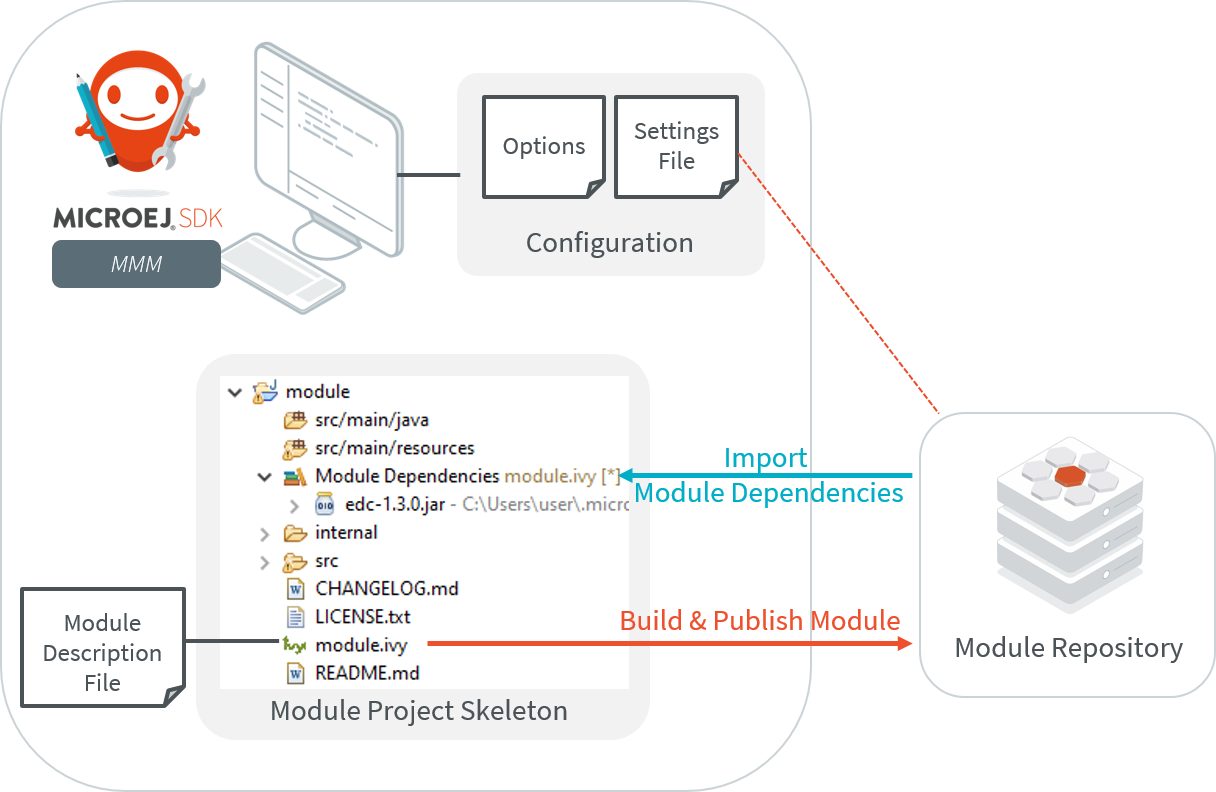
\includegraphics[width=.8\textwidth]{./ressources/schemas/mmm_flow.png}
\end{center}

\section{Interactions internes}

\subsection{WTM}

La Weekly Tech Meeting est une réunion hebdomadaire permettant un partage de l’avancement de chaque projet en cours. Cela permet d'augmenter la cohésion des équipes et aussi de présenter les évolutions des outils internes qui peuvent potentiellement être utilisés par tous.

\subsection{RocketChat}

En particulier avec le confinement il est capital d’avoir un outil permettant des échanges écrits. L'entreprise utilise \href{https://rocket.chat/}{Rocketchat}. Ce programme offre deux services : des salons qui permettent des échanges entre des groupes de personnes autour d'un sujet précis et des conversations privées.

Le chat est hébergé dans le réseau de l’entreprise, il est donc nécessaire de se connecter avec le VPN pour y accéder. Le contenu des messages est considéré comme privé par défaut.
Ce chat est très utile car il permet, de communiquer des informations liées :

\begin{itemize}
\setcounter{enumi}{-1}
\item aux ressources humaines
\item aux projets en cours
\item aux problèmes rencontrés
\end{itemize}

En effet, la résolution de problèmes passe par le chat et l'appel aux compétences des autres informaticiens de l’entreprise. Chaque projet pouvant présenter des problèmes particuliers suivant les capacités et versions des plateformes utilisées, il serait trop long de tous les répertorier. Il serait par contre dommage de perdre du temps en n’utilisant pas les connaissances accumulées dans l’entreprise, d'où l'utilité du chat. 

\subsection{IT support}

Lorsqu’un problème est lié aux outils personnels tel que les sessions ou le matériel emprunté, une plateforme de support dédié GLPI permet de contacter ‘formellement’ par des tickets la personne chargée du support.

\section{Interactions externes}
\subsection{Site Principal}

\href{https://www.microej.com/}{Le site principal de MicroEJ} sert de vitrine pour l'entreprise et ses produits. Il contient aussi les informations de contacts pour le public.

\subsection{Site développeur}

\href{https://developer.microej.com/}{Ce site} contient de nombreux tutoriels allant de la mise en place d'un environnement de développement pour la VEE MicroEJ, à la création d'applications et jusqu'à l'analyse des performances et l'optimisation des programmes.

\subsection{Documentation publique}

\href{https://docs.microej.com/en/latest/}{La documentation publique} contient les informations nécessaires pour le développement d’applications sur l’IDE MicroEJ SDK.

\subsection{Forum dev}

Ce forum public permet des échanges entre les développeurs utilisant la plateforme MicroEJ et les développeur chez MicroEJ. Ce forum a aussi un rôle de guide développeur secondaire. Il permet de poser des questions techniques aux personnes travaillant dans des ‘setups’ similaires et ayant beaucoup plus de chance d’avoir déjà rencontré le problème et de connaître sa solution.

\subsection{Github MicroEJ}

\href{https://github.com/MicroEJ}{Ce Github} public contient des exemples d’applications sur la MicroEJ VEE. Il contient aussi la documentation développeur ce qui permet de la modifier simplement dès que l'on détecte un problème pendant son utilisation.

\section{Simple application with GUI}

Une partie importante de la procédure newcomers est la création d'une application graphique en utilisant les ressources et l'IDE MicroEJ comme un développeur externe le ferait. 
J'ai décidé de créer une application qui afficherait la date, l'heure et la météo d'une ville sélectionnée. Cette application nécessitant plusieurs écrans et composantes, j'ai pu me familiariser avec le framework widget de MicroEJ permettant de construire ce genre d'interfaces.

Pour le développement j'ai utilisé l'IDE MicroEJ SDK. Cet IDE basé sur Eclipse contient des outils permettant l’exécution d'applications MicroEJ sur des cartes électroniques physiques ou simulées.

\subsection{Horloge}

La première étape était de se familiariser avec le framework d’applications de MicroEJ. Celui-ci permet de créer des applications pouvant être lancées/arrêtées/chargées sur l’environnement sandboxed de MicroEJ. 

Ce framework contient un système de tâches pouvant être déclenchées à intervalles réguliers.
Cela m’a aussi permis de me familiariser avec l’utilisation de polices autres que celle par défaut. La plateforme MicroEJ se voulant la plus légère possible, les polices doivent être ajoutées manuellement et si possible uniquement les caractères nécessaires. Dans mon cas j’ai pu utiliser pleinement cette fonctionnalité en ne chargeant que les chiffres et lettres nécessaires pour afficher une date. 

\subsection{Météo}

Le relevé météorologique était récupéré sur l’API en ligne \href{https://openweathermap.org/}{OpenWeatherMap}. Ce site propose une offre gratuite avec un maximum de 60 requêtes par minute ce qui est suffisant pour une démonstration. L’API est questionnée par une requête http GET. On peut donc générer une chaîne de caractères à envoyer simplement en java. La réponse est une chaîne de caractères dans plusieurs formats possibles (XML,JSON…).Dans mon cas j’ai utilisé le résultat en JSON car une librairie MicroEJ traitant le format JSON existait déjà. 
Une fois les informations météorologiques récupérées j’ai pu passer à l’affichage. L’affichage de la météo m’a permit de me familiariser avec l’utilisation d’images dans les applications MicroEJ. 

\subsection{Icônes météo}

J'ai créé des icônes permettant de représenter la météo :

\begin{center}

\includegraphics[width=.5\textwidth]{./ressources/images/weathertogether.png}
\end{center}

Ces icônes sont ensuite assemblées pour rendre compte des différentes conditions météorologiques.

L'écran principal était complété :

\begin{center}
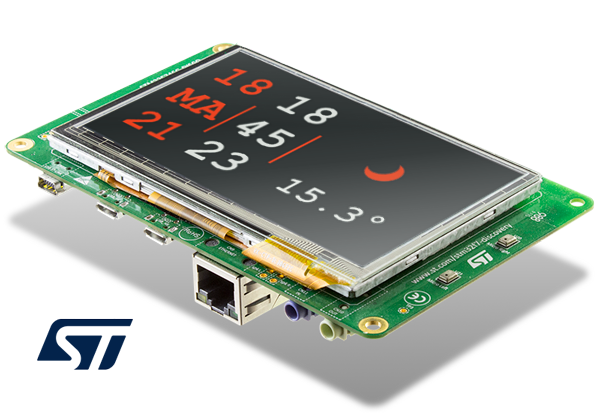
\includegraphics[width=.5\textwidth]{./ressources/schemas/inSituation.png}
\end{center}

\subsection{Menu choix ville}

Pour finir le programme il m’a fallu créer un écran permettant la sélection d’une ville, modifiant dynamiquement la timezone et la météo. Cela a nécessité de porter le programme vers une structure en widgets dans laquelle on puisse passer d’un widget/écran à l’autre puis interagir avec chaque écran.
Le framework widget de MicroEJ permet de créer des widgets composées d’autres widgets. J'ai pu récupérer un widget clavier sur un projet existant et l’intégrer au widget de sélection. 

\begin{center}
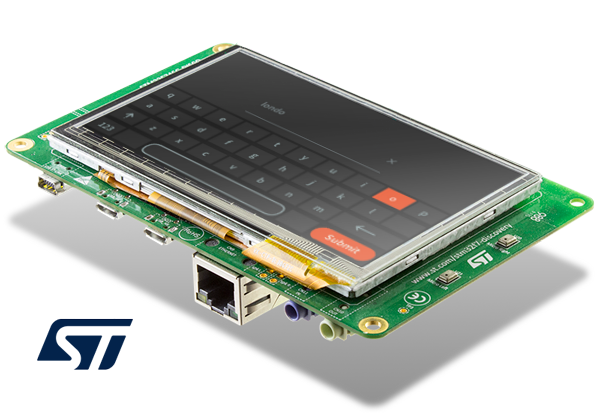
\includegraphics[width=.5\textwidth]{./ressources/schemas/inSituationSel.png}
\end{center}

\subsection{Finalisation}

J'ai ensuite continué à retoucher ce projet en parallèle du Dependency Discoverer. Cela a compris l'ajout de variations de la couleur de fond de l'horloge en fonction de la position du soleil afin de rendre compte de l'aube et du crépuscule. J'ai aussi rédigé un README qui présentait les fonctionnalités de l'application et les dépendances sur lesquelles elle repose.

\begin{center}
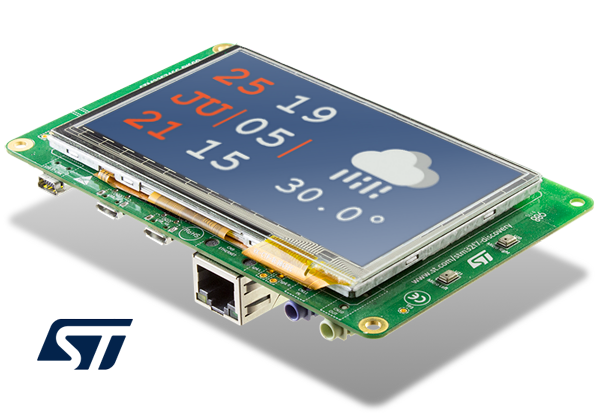
\includegraphics[width=.5\textwidth]{./ressources/schemas/inSituationFin.png}
\end{center}


\chapter{Dependency Discoverer}

\section{Présentation du sujet}

Le produit principal de MicroEJ est le MicroEJ VEE :

\begin{center}
  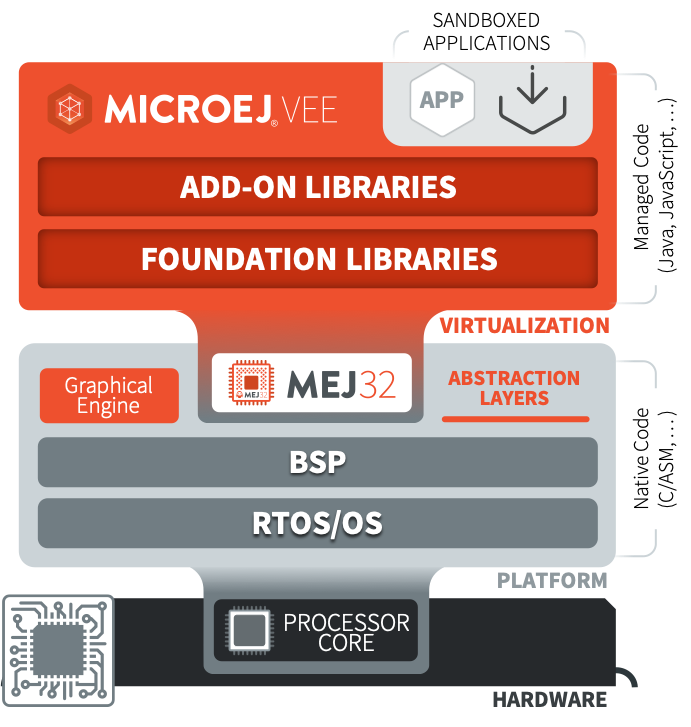
\includegraphics[width=.6\textwidth]{ressources/schemas/Implementations-on-hardware_minimize.png}
\end{center}

Comme on peut le voir illustré ci-dessus, ce programme permet l’interface entre le kernel de la carte électronique et les applications en virtualisant un environnement commun quelle que soit la carte, reposant sur l’architecture virtuelle MEJ32. Afin de respecter les exigences matérielles, de nombreuses librairies Java ont été allégées afin d’offrir la même API pour de meilleures performances. Les foundation libraries contiennent les librairies communes à tous les projets tandis que les add-on librairies doivent être importées lors du développement afin d’être intégrées au VEE lors de l’exécution sur carte.

Lorsqu’un client veut porter une application existante il peut vouloir utiliser des librairies qui n’ont pas encore été recodées pour une utilisation dans la VEE MicroEJ. Dans ce cas il est important de déterminer rapidement quelles sont ces librairies et si un remplacement par des librairies existantes est possible. Sinon il faudra que ces librairies soit développées par MicroEJ ce qui aura un coût. Cette information est donc cruciale pour les futurs clients.
 
Le Dependency Discoverer répond à ce besoin en listant automatiquement toutes les APIs dont le programme testé dépend et qui n’ont pas encore été portées pour le MicroEJ VEE. Cela se fait en listant toutes les dépendances puis en retirant celles présentent dans une liste de fichiers jar nommée againstClasspath. Liste pointant sur les jars du dépôt de librairies MicroEJ téléchargé automatiquement. Pour plus de simplicité le programme est accessible directement par les clients. Cet outils nécessite cependant une refonte pour deux raisons principales :

\begin{itemize}

\item La librairie permettant l’analyse des programmes est bloquée à JAVA 7 induisant une obsolescence qui à déjà été rencontrée.

\item La politique de MicroEJ étant plus ouverte à l’open source le Dependency Discoverer doit être passé totalement en open source là ou le programme d’analyse était en closed source.
Cette refonte s’est faite en plusieurs étapes distinctes permettant d’atteindre ces objectifs.

\end{itemize}

\section{Passage à ASM }

Le fonctionnement du Dependency Discoverer repose sur l'analyse des fichiers class qui contiennent le programme compilé. 

\bigskip

\subsubsection{fichiers java}

Le code édité par le programmeur est enregistré dans le format JAVA :

\begin{lstlisting}

public class TestASM {
	
	public String testStringDependency(){
		return "this is a test";
	}
	
}

\end{lstlisting}

Ce code est ensuite compilé pour exécution dans le format class aussi appelé \textit{bytecode}. Ce format n'est pas affichable tel quel mais la commande javap permet d'en récupérer le contenu :

\begin{lstlisting}

public class TestASM {
  public TestASM();
  public java.lang.String testStringDependency();
}


\end{lstlisting}

C'est ce format qui est analysé par le Dependency Discoverer. On remarque qu'il manque des informations dans l'affichage standard du fichier class avec javap. L'ajout du flag -v permet un \hyperref[javapVtestASM]{affichage complet}. Il contient même plus d'informations que dans le code non compilé comme la méthode d'initialisation qui est héritée de java/lang/Object.

\bigskip

L'ancienne version utilisait une librairie d'analyse interne à l'entreprise, limitée à la version 7 de Java. Maintenant que la majorité des programmes créés le sont dans une version supérieur ou égal à Java 8 il est nécessaire de changer de librairie. J'ai utilisé une librairie open source déjà existante : \href{https://asm.ow2.io/}{ASM}. Cette librairie fiable permet l'analyse et l'édition de bytecode et est utilisée par les compilateurs Gradle et Kotlin ainsi que par la JVM pour certaines opérations effectuées pendant l’exécution du code.

Pour effectuer le passage à ASM, j'ai dû comprendre l'intégration de l'ancienne librairie d'analyse afin de modifier tous les appels par son API pour les remplacer par des appels à l'API d'ASM. Cela a aussi nécessité de comprendre le pattern visiteur sur lequel les deux librairies reposaient pour l'itération à travers le code. ASM charge les fichiers class dans une hiérarchie de nœuds dont la base est constituée de variables de type \textit{Classnode}. L'outil de debug d'Eclipse m'a permis de lire le contenu de ces variables et de me rendre compte de la \hyperref[ClassNode]{complexité de la structure}.

\bigskip

\subsubsection{\textit{Pattern visiteur}} 

\textit{Ce pattern de programmation répond au besoin d'analyser différemment une structure complexe de données sans avoir à réécrire une série de méthodes dédiées.}

\textit{Pour cela on met en place un visitable et un visiteur. Le visitable contient la structure de données et possède une méthode prenant en paramètre un visiteur; durant l’exécution de cette méthode, le visitable va itérer à travers toute la structure de données et appeler, pour chaque donnée, une méthode du visiteur permettant son traitement.}

\textit{Java permet l'override : une classe fille héritant d'une classe mère peut redéfinir le contenu d'une méthode. Une classe fille d'un visiteur peut donc être passée en paramètre du visitable correspondant et appliquer un traitement personnalisé des données .}


\bigskip

Pour l'analyse il faut lister les méthodes des Classnodes puis créer une classe qui hérite du visiteur de méthodes standard ASM pour effectuer une visite dans ces nœuds de méthode (seul le code référencé depuis des méthodes sera vraiment exécuté et nécessite une analyse). On peut ensuite réécrire le contenu de ces fonctions pour appeler les nôtres. Dans mon cas j'ai appelé les méthodes existantes permettant de rajouter des dépendances.   

Cette tâche a nécessité un travail de recherche sur internet et dans la documentation d’ASM ainsi que d’appliquer mes compétences en programmation afin de comprendre et modifier le code. \hyperlink{competences}{TC.2.4}.

\section{Open source ready}

Le Dependency Discoverer était originellement séparé en deux parties, une dont le code était accessible publiquement permettant d'utiliser le programme et une autre, compilée sous la forme d'un jar contenant l'outil d'analyse. Une partie de mon sujet était donc de réunir les deux parties du programme.

Pour ce faire j'ai pris connaissance du code, en particulier du Framework faisant l'interface entre les deux parties du programme. J'ai pu ensuite supprimer les classes et interfaces inutiles tout en vérifiant le bon fonctionnement avec les tests unitaires Junit déjà mis en place.

\subsection{Junit}

Junit est un framework de test de code utilisé sur l’IDE MicroEJ SDK. Les tests sont effectués autour du programme, ce qui signifie que tant que les API du programme ou d'une partie du programme testé restent les mêmes, les tests sont toujours valides et permettent d’évaluer si un changement dans le code casse une fonctionnalité.

\begin{center}
 	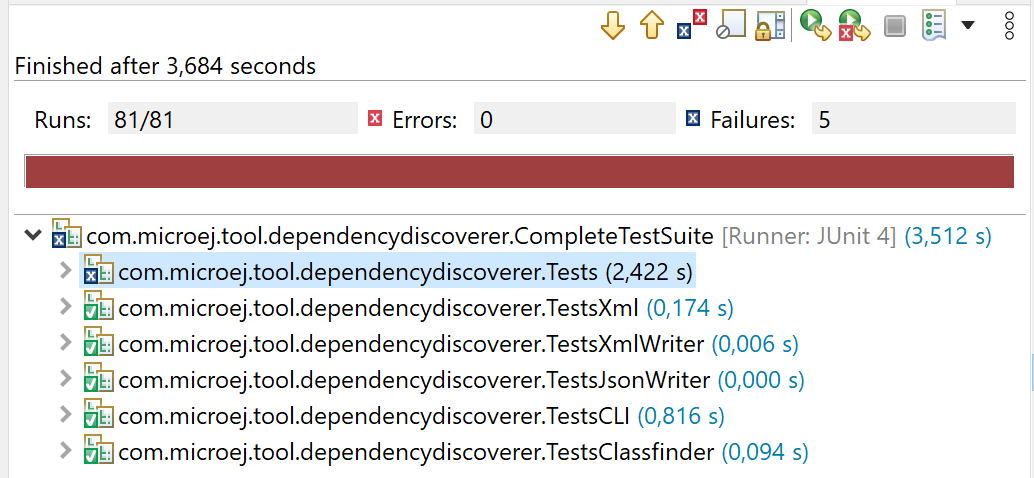
\includegraphics[width=\textwidth]{ressources/images/junit.png}
\end{center}

on peut voir que certains tests ne passent pas. Ils sont liés à l'analyse d'un cas particulier où une dépendance n’apparaît que pendant l’exécution. S'assurer que le problème ne survienne jamais est donc impossible car le Dependency Discoverer effectue une analyse statique du code. Le test est donc laissé pour indiquer que le programme possède des exceptions.

\subsection{CLI}

Originellement, l'utilisation du Dependency Discoverer nécessitait de charger le code source dans une variation de l'IDE Eclipse et de l’exécuter dans cet IDE. Cette solution n'est pas pratique, en particulier pour un client externe à l'entreprise. Une \hyperlink{CLI}{CLI} est bien plus adaptée.

Interfacer un programme Java pour un appel par une interface en ligne de commande nécessite l’utilisation d’une librairie dédiée. Mon tuteur avait choisi \href{https://picocli.info/}{picocli}, une librairie très complète, avec une excellente documentation et déjà utilisée dans d'autres projets. Une classe permettant d’interfacer le programme existait déjà pour utiliser l’archive contenant le code close source. J’ai donc repris cette classe comme base. 

L’implémentation de picocli était simple grâce à la documentation. Il fallait juste prendre le temps de choisir des options pertinentes avec des noms clairs pour l’utilisateur. L’outil génère automatiquement une page d’aide du programme accessible avec l’option ‘--help’. Cela permet de créer facilement une description customisée.

\section{Code quality}

Le code allant être posté publiquement il est d’autant plus nécessaire qu’il ne contienne aucun code smell car d’autres personnes vont y accéder et potentiellement essayer de l’améliorer. Pour les y aider, le code doit être le plus lisible et propre possible . Cela permet aussi de promouvoir le sérieux de l’entreprise. 

\subsection{Code smells}

Pour supprimer les 'code smells' c'est-à-dire les lignes au comportement incertain ou pour lesquelles un remplacement plus efficace ou élégant existe, j'ai utilisé SonarLint.

SonarLint permet de faire de l’analyse de code au vol. Cet outil renseigne sur tous types de problèmes : de codes pouvant provoquer une erreur à du code mal optimisé ou peut lisible avec une explication du problème ainsi que des exemples de corrections.
L'IDE MicroEJ SDK contient SonarLint ainsi que les règles suivies par l'entreprise.

\subsection{Null Analysis}

Un autre angle d'amélioration du code est la null analysis qui consiste en la systématisation du traitement des variables nulles. On pourra donc prévenir les tentatives d'accès à des valeurs nulles qui feraient quitter le programme sur une erreur. 

Le mécanisme utilisé est un système d'annotations (@NonNull et @Nullable) à placer dans le code permettant à l'IDE de déterminer lorsqu'un accès invalide peut survenir. On renseigne le fichier package-info.java dans chaque paquet Java pour mettre @NonNull comme annotation par défaut :

\begin{lstlisting}
@org.eclipse.jdt.annotation.NonNullByDefault
package packagename;
\end{lstlisting}

On peut ensuite rajouter l'annotation @Nullable quand on a besoin qu'une variable puisse passer dans l'état null. L'IDE va ensuite automatiquement prévenir l'utilisateur des accès à cette variable avant instanciation.

\begin{center}
  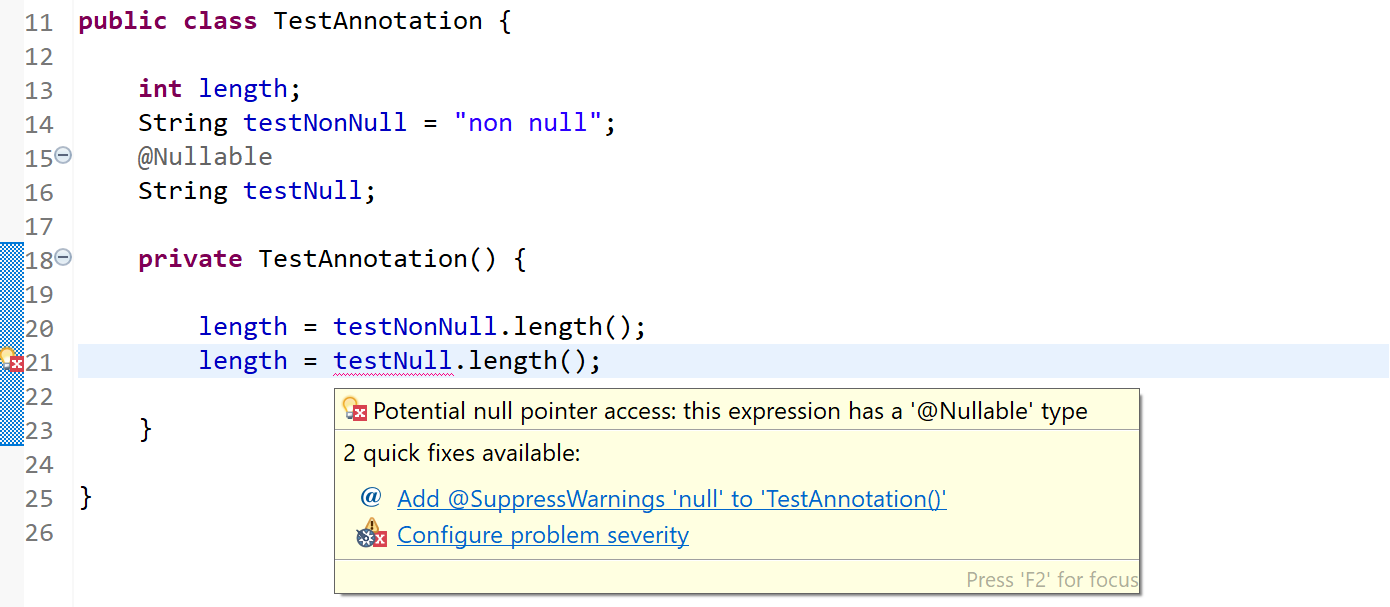
\includegraphics[width=\textwidth]{ressources/images/nonnull.png}
\end{center}

La majorité des programmes conçus chez MicroEJ le sont sous la version 7 de java, les null analysis aussi. Le système d'annotation du programme pour effectuer la null analysis a cependant été modifié à partir de la version 8 et a perdu toute rétro-compatibilité. Cette incompatibilité n'a été détectée par mon tuteur que lorsqu'il a voulu vérifier mon code avec sa configuration en Java 7. Nous avons donc tous les deux fait des recherches et tests afin d'établir la liste des changements à opérer pour passer de la version 7 à la version 8. 
Cela a permis de résoudre le problème pour d'autres projets sous Java 8+.

Après ça j'ai pu finir l'analyse en utilisant les fonctionnalités de la version 8, non sans difficultés. L’outil est en effet rarement utilisé et la documentation officielle est trop sommaire et ne couvre que certains cas généraux. Certaines annotations doivent être renseignées à part sur des fichiers particuliers et l'IDE pouvait parfois nécessiter d'être rechargée voir relancée pour mettre à jour les changements d'annotations. Ces fichiers doivent être écrits dans un format unique, sans possibilité d'avoir une aide à la correction et peuvent ne pas fonctionner pour un espace en trop. J'ai donc utilisé un programme de test afin de créer ces fichier dans un environnement plus contrôlé.

Pour exemple : la méthode get de la classe HashMap. Cette classe fait partie des librairies Java ; elle ne peut donc pas être modifiée, les annotations doivent donc êtres externes. Cette méthode nécessite des annotations car par défaut @NonNull est utilisé pour des librairies externes. Or cette méthode peut renvoyer null et ce, même si toutes les autres valeurs sont non null : une Hashmap est similaire à un dictionnaire : même si le dictionnaire ne contient que des mots et définitions valides mais que le mot que l'on cherche n'y est pas présent on ne récupérera aucune définition.

Pour la fonction suivante on passe de l’entête :
\begin{lstlisting}
public V get(Object key);
\end{lstlisting}

au fichier d’annotations externe au format eea :

\begin{verbatim}
class java/util/HashMap
get
 (Ljava/lang/Object;)TV;
 (L0java/lang/Object;)T0V;
\end{verbatim}

pour indiquer que les variables d'entrée et de sortie peuvent être nulles.

Enfin j'ai rédigé un tutoriel sur l'utilisation des annotations en Java 8+ afin de partager mes connaissances acquises avec toutes les personnes qui auront à travailler avec au sein de MicroEJ.

\subsection{Éxecutable Windows}

Les programmes Java nécessitent d’être exécutés par une machine virtuelle Java. Ce programme est lancé avec le Dependency Discoverer et va énormément ralentir le lancement. De plus, utiliser le Dependency Discoverer nécessite d’avoir cette JVM installée. La solution la plus rapide et simple pour l’utilisateur est d’avoir un seul programme exécutable contenant tout le code nécessaire. Étant donné que la plupart des utilisateurs seront sur Windows je me suis concentré sur un exécutable pour cette plateforme.

La documentation de picocli conseille l’utilisation de l’outil \href{https://www.graalvm.org/}{GraalVM} pour la création d’exécutables. GraalVM assure la compatibilité avec picocli et la création d’un exécutable indépendant de la présence d'un interpréteur Java en générant une JVM allégée et adaptée au programme. 

Utiliser GraalVm ne nécessite aucune modification dans le code. J’ai suivi la documentation officielle afin de générer l’exécutable. Celle-ci étant complète je n’ai rencontré aucun problème pour créer un premier exécutable permettant de faire une ‘proof of concept’.


\section{Automatic build}

\subsubsection{Build platform}

\textit{Le but d’une build platform est de récupérer automatiquement le code source d’un programme pour effectuer différentes opérations permettant de vérifier la qualité et le bon fonctionnement du programme. Les plateformes de build sont au centre de la CI}

\subsection{Proof of concept}

Mon objectif était d'utiliser un service offrant la possibilité de tester le programme, générer un exécutable jar (pour une exécution sur toutes les plateformes via Java) et exe (pour une exécution sur Windows sans environnement d’exécution Java) et enfin poster ces exécutables sur Github. 

Le code est hébergé sur un dépôt Github public, par conséquent il était nécessaire d’utiliser une plateforme de build externe, pour être exact \href{https://travis-ci.com/}{Travis CI}. Cette plateforme avait été repérée par mon tuteur pour de futurs projets, nous avons donc profité de l'ouverture à l'open source du Dependency Discoverer pour tester si cette plateforme conviendrait.

Afin de générer automatiquement un exécutable Windows il est nécessaire d’utiliser Windows comme plateforme de build. Ce service est assez récent ce qui implique:

\begin{itemize}

 \item que les options ne sont pas toutes disponibles
 \item que peu d’exemples existent
 \item que la documentation n’est pas complète.

\end{itemize}

Après de plus amples recherches j’ai trouvé un exemple d’utilisation de la plateforme pour créer un exécutable à partir d’un programme Java. Cette base contenait toutes les instructions nécessaires pour l’installation des outils de builds. J’ai pu ensuite adapter les commandes que j’avais utilisées pour effectuer le build sur mon pc, sur un projet de test consistant en un simple programme calculant la décomposition en nombres premiers d'une valeur entière d'entrée.

La dernière étape était l’envoi du résultat sur Github ; cela a nécessité beaucoup d'essais pour avoir un envoi fonctionnel. Le plus gros problème a été la création de variables sécurisées. Toutes les informations requises au build sont renseignées sur un fichier compris dans le projet Github, ce qui signifie qu’il est lui aussi ‘open source’. L’e-mail , le nom et le jeton d’envoi sont donc eux aussi disponibles publiquement... N’importe qui pourrait donc récupérer ce jeton pour modifier le code. La solution proposée par TravisCI est la possibilité de chiffrer ces informations qui seront déchiffrées mais cachées pendant le build. La solution la plus simple pour chiffrer des informations est d’utiliser le programme dédié, disponible pour les plateformes Linux. Étant sur Windows il m’a donc fallu mettre en place un environnement virtuel Linux.

\subsubsection{\textit{Multi-plateform setup}}

\textit{Rares sont les programmes proposant des versions pour tous les systèmes d’exploitation majeurs. Il est donc parfois nécessaire d’utiliser plusieurs systèmes d’exploitations pour avoir accès à tous les programmes dont on a besoin. Il est cependant impossible d’avoir 3 ou 4 machines différentes ou de redémarrer son ordinateur plusieurs fois par jours pour changer d’OS. La solution : avoir un système d’exploitation duquel on pourra lancer les autres systèmes par virtualisation. Pour cela j’ai utilisé WSL.}

\subsubsection{\textit{WSL}}

\textit{WSL est un environnement virtuel permettant de lancer un système Linux sur Windows avec un terminal pour seule interface. Cette solution est donc assez légère mais la propriété la plus intéressante est la possibilité pour le système Linux d’accéder au système de fichiers Windows. Cela permet donc d’exécuter des programmes Linux directement dans le système Windows sans avoir à copier les fichiers dans l’environnement Linux.}\\

J’ai utilisé une image Ubuntu, la distribution Linux la plus complète actuellement disponible. Une fois WSL mis en place j’ai pu générer les variables sécurisées sur mon projet d'expérimentation. Après avoir vérifié la page release sur Github les fichiers uploadés sont bien présents.

\begin{center}
  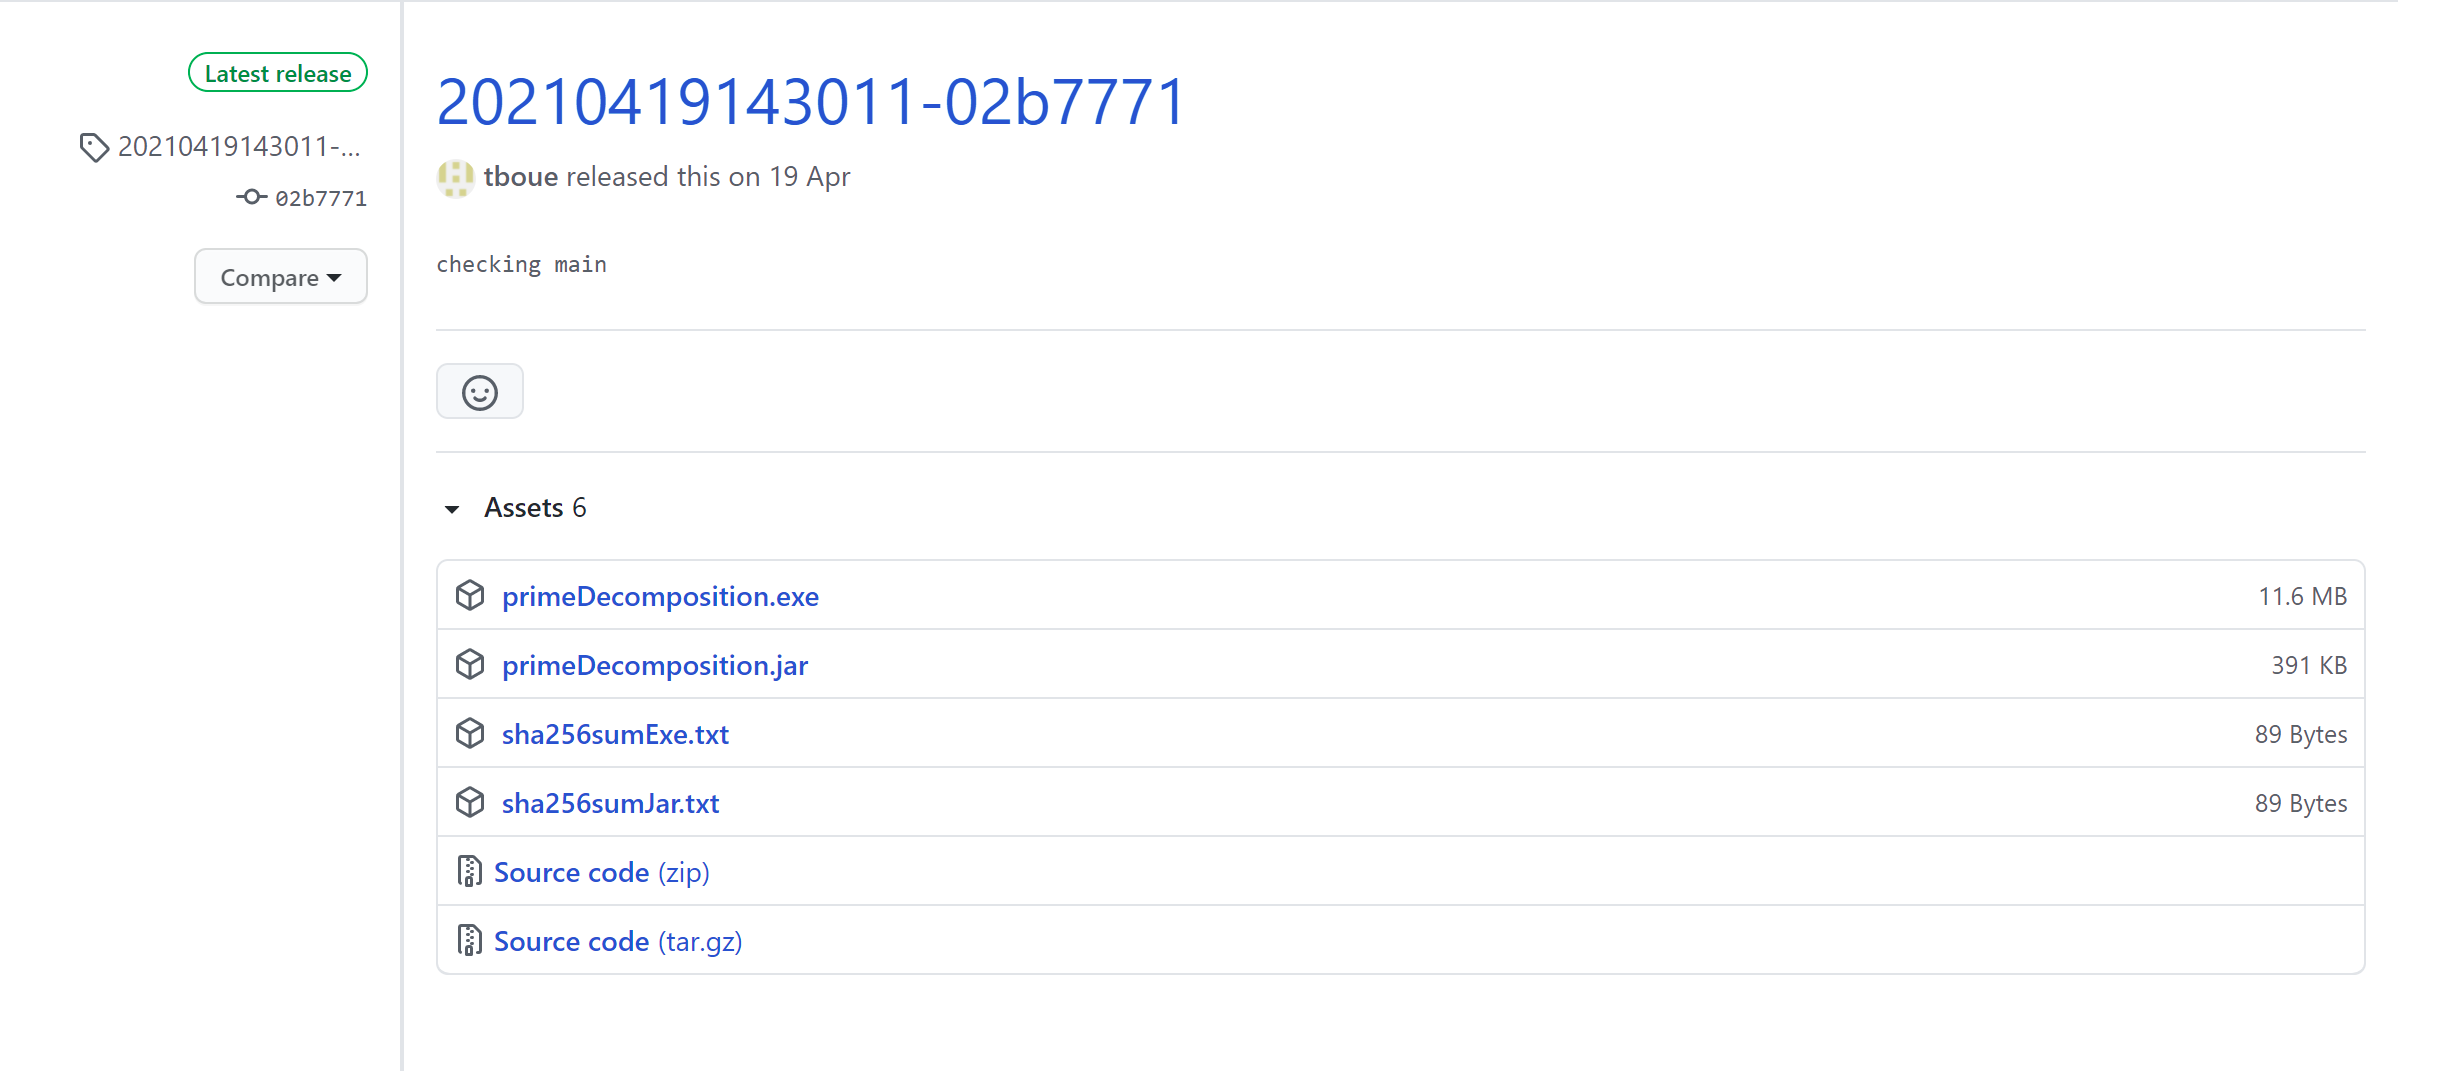
\includegraphics[width=\textwidth]{ressources/images/github.png}
\end{center}

J'ai pu télécharger les fichiers et utiliser la Powershell Windows pour vérifier le bon fonctionnement de l’exécutable de mon projet de test généré automatiquement:

\begin{center}
  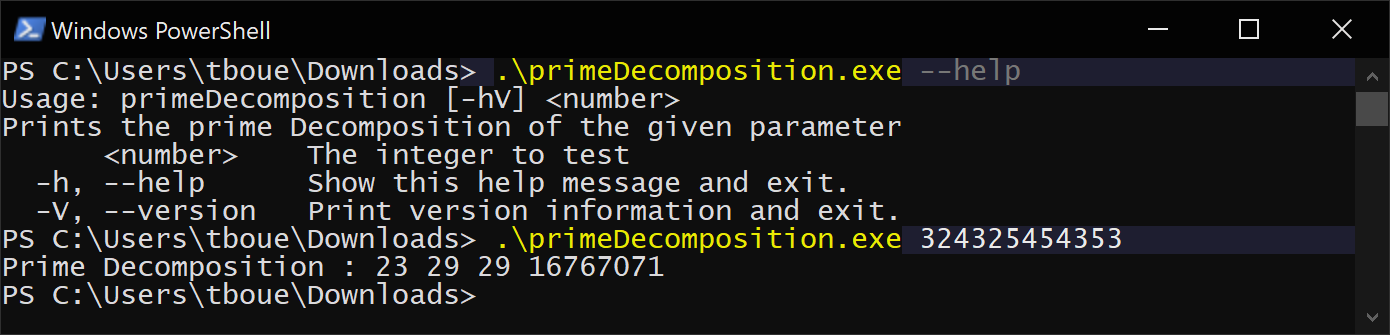
\includegraphics[width=\textwidth]{ressources/images/exePrime.png}
\end{center}

J'ai enfin créé une copie du projet du Dependency Discoverer sur un Github privé pour adapter le build à ce projet.

\subsection{Build automatique 2 : Junit}

Après avoir démontré la faisabilité d’un build sur la plateforme TraviCI il m’a fallu créer le script final qui intégrerait les tests Junit. De cette façon n’importe qui reprenant le programme plus tard pourra modifier le code sans risquer de le poster avec des fonctionnalités cassées.

Intégrer les tests a été assez simple car de nombreux exemples de tests Junit sur la plateforme Ant existaient. Seulement trois tests ont été nécessaires. Cependant le résultat du test était différent sur la plateforme de build et en local. Ce problème est assez commun pour les plateformes de build, l’environnement étant différent de celui de développement. Il fallait donc trouver les différences de configurations et/ou de librairies.

Après avoir testé plusieurs programmes et configurations de build sans modifier le résultat j’ai décidé de prendre le problème à l’envers.

Je me suis en effet rendu compte en comparant des codes compilés avec l’outil de build et le MicroEJ SDK que la différence de résultat était provoquée par une différence de code dans les fichiers compilés de test (tout le code était compilé différemment mais le fonctionnement à l’exécution était le même). Ayant réduit mes recherches à des classes de quelques lignes j’ai pu inférer les différences de configuration et résoudre ce problème.

Je me suis donc intéressé au format .class correspondant aux classes compilées Java. 
Après comparaison j’ai identifié la différence : la présence de lignes de code utilisées lors d'une exécution en mode debug dans l’IDE. Après ajout de l’option activant cette fonction le build est passé.

\subsection{Automatic build 3 : Évaluation des Github Actions}

Les outils informatiques évoluent et peuvent passer de gratuits à payants et inversement. Une formule classique des services informatiques est d’avoir une option gratuite mais limitée, permettant une utilisation pour des démonstrations, des projets amateurs ou des projets open sources. La dépendance à un service payant est un frein majeur à l’open source. Notre projet, étant open source, une solution gratuite de ce type correspondrait et Travis CI la proposait jusqu’en 2018. La société a ensuite changé de politique après un rachat. La nouvelle formule est une solution payante pour laquelle chaque nouvel utilisateur a un certain nombre de crédits de base. Pour être exact 1000 crédits correspondant à 100 minutes d’utilisation de la plateforme. Soit environs 25 builds avec la version complète du build. L'ancienne formule est toujours accessible pour les projets open source mais uniquement sous réserve de l'acceptation de la plateforme après présentation d'un dossier.

L’objectif pour mon tuteur était que je crée une proof of concept de l’utilisation de Travis CI pour tous leurs projets open-source. Ce genre de limitations pousse donc à évaluer d'autres solutions.

Une possibilité serait d’utiliser une plateforme proposant une formule toujours gratuite comme Github action. Celle-ci a aussi l’avantage d’être intriquée à Github . Elle est par contre moins aboutie et après recherche, risque de nécessiter un plus grand investissement en R\&D pour mettre au point le build automatique et ce, sans assurance d’effectivement atteindre ce résultat.

La solution Travis CI a donc été gardée pour le moment mais lorsque ce sera possible, un passage sur Github action sera sûrement effectué.

\section{Documentation}

Le programme modifié, la documentation devait être mise à jour pour correspondre à la nouvelle interface et les nouvelles possibilités d’utilisation.

\subsection{Javadoc}

Cette documentation interne au programme est différente des commentaires eux qui donnent des informations sur des lignes de code. La Javadoc est destinée aux variables et méthodes publiques, plus généralement, aux APIs. Cette documentation est donc destinée aux futurs développeurs voulant travailler autour de ces APIs sans avoir à lire le code.

\subsection{README}

La documentation est rédigée dans deux formats : md et rst. Un tutoriel local chez MicroEJ contient toutes les guidelines pour rédiger ces fichiers. J'ai repris l'ancien README et ai rajouté la marche à suivre pour utiliser le programme par la CLI. J'ai aussi modifié la liste des options en copiant celle donnée par la CLI. 

\section{Junit CLI}

Au cours du développement, la CLI a gagné en complexité et des tests unitaires devenaient nécessaires pour s’assurer que le comportement soit celui attendu. Ces tests portent uniquement sur les différentes combinaisons d’options possibles. 

Les options sont passées en argument des programmes Java via la méthode static main. Une fois cette méthode terminée le programme et la JVM quittent. On ne peut donc pas appeler cette fonction directement de Junit car, à la sortie de la première méthode main, la suite de tests quittera au premier test avec la JVM. 
L’implémentation de picocli m’a permis d’effectuer les tests. Celle-ci fonctionne comme suit : la méthode main appelle L’API picocli avec en argument, une instance de la classe principale DependencyDiscovererCLI, ainsi que les arguments passés dans le main.
Picocli va alors appeler la méthode run de l'objet DependencyDiscovererCLI avec les arguments du main. Le main est donc appelé sur l'interface picocli mais pas sur le Dependency Discoverer.
En reproduisant cet appel sur run on peut donc reproduire l’appel du programme avec des arguments sans passer par la méthode main.
Pour récupérer le résultat du traitement de la méthode run de la classe DependencyDiscovererCLI on transforme la classe pour enlever les variables statiques (même valeur pour tous les objets créés) afin d’avoir une complète indépendance des tests. On rajoute ensuite des méthodes pour récupérer les valeurs et les comparer aux valeurs attendues.

Les tests ont révélé des problèmes de conception, majoritairement des options rentrant en conflit ou n’ayant pas le comportement attendu. Parmi tous ces problèmes l'un m’a pris plus de temps à résoudre. Entre deux tests, il m’était impossible de supprimer les fichiers jar utilisés pour l’analyse. Ce problème montre que produire du code qui respecte les règles proposés par SonarLint, et pas seulement fonctionnel, a un intérêt : 
lors de l'analyse, les fichiers jar n'étaient pas refermés correctement. Lorsque le programme était lancé normalement ces fichiers restaient ouverts le temps que le résultat soit retourné puis étaient fermés avec la JVM. Sauf que pour les tests, la JVM ne se coupe pas entre chaque analyse : les jar restent donc ouverts jusqu’à la fin des tests. 
La fermeture des fichiers après utilisation est une règle basique mais il peut parfois être compliqué de suivre le flow du programme et déterminer quand opérer cette fermeture.

\section{Sortie JSON}

Le programme pouvait renvoyer le résultat sous deux formats :

\subsubsection{texte}

\begin{lstlisting}
java/awt/Color
java/awt/Coror.RED
java/awt/Color.<init>(I)V
\end{lstlisting}

\subsubsection{XML}

\begin{lstlisting}[language=xml]
<?xml version="1.0" encoding="UTF-8"?>
<require>
	<type name="java.awt.Color">
	<field name="java.awt.Color.RED">
	<method name="java.awt.Color.Color(int)void">
</require>
\end{lstlisting}



J'ai rajouté une sortie au format JSON ainsi que les tests Junit nécessaires à la vérification du bon fonctionnement des méthodes d'écriture.

\begin{lstlisting}
{
	"require":{
		"type":[ 
			{
				"name":"java.awt.Color"
			}
		],
		"field":[
			{
		 		"name"="java.awt.Color.RED"
		 	}
		 ],
		"method":[
			{
				"name"="java.awt.Color.Color(int)void"
			}
		]
	}
}
\end{lstlisting}

Ce format peut être traité par de nombreuses librairies dans divers langages de programmation et permet de multiples possibilités d'intégration du Dependency Discoverer.


\section{Optimisations}

L’optimisation est une étape particulière du développement d’un programme. Optimiser un programme revient souvent à le rendre moins lisible et surtout à limiter ses capacités pour qu’il n’effectue que les tâches nécessaires à son fonctionnement. Diagnostiquer des problèmes d’optimisation nécessite aussi des tests plus larges en conditions réelles . D’un point de vue général l'optimisation est donc effectuée en dernier. 
Les premiers tests sur des projets récents ont révélé que le Dependency Discoverer était très lent et que le temps d’exécution augmentait rapidement, proportionnellement au nombre de dépendances. 

J’ai mis en place un test du temps d’analyse sur un programme comprenant 32 dépendances à détecter. Ce test était beaucoup plus réaliste même s'il n'était pas encore au niveau des conditions rencontrées dans des projets de grande ampleur. Malgré tout, le nombre de dépendances était déjà assez important pour constater le problème, l’analyse prenait 25 secondes. Donc jusqu’à plusieurs minutes pour un programme plus complet. Après vérification l’ancienne version du Dependency Discoverer renvoyait un temps d’exécution similaire : il allait donc falloir analyser tout le code car la lenteur n'avait pas été introduite avec un des changements que j'avais effectué.

\subsubsection{VisualVM}

Pour diagnostiquer d’où venait cette lenteur j’ai utilisé l’outil \href{https://visualvm.github.io/}{VisualVM} .Celui-ci est majoritairement utilisé afin d’analyser l’utilisation mémoire des programmes Java pour trouver des fuites mémoire (j’avais d’ailleurs utilisé ce programme pour la première fois pour une analyse de la mémoire d’un programme Java d'un projet personnel). Il offre cependant aussi la possibilité de relever le temps passé dans chaque méthode d’un programme. J’ai donc généré un rapport pour le Dependency Discoverer.

\subsection{Analyse}

\begin{center}
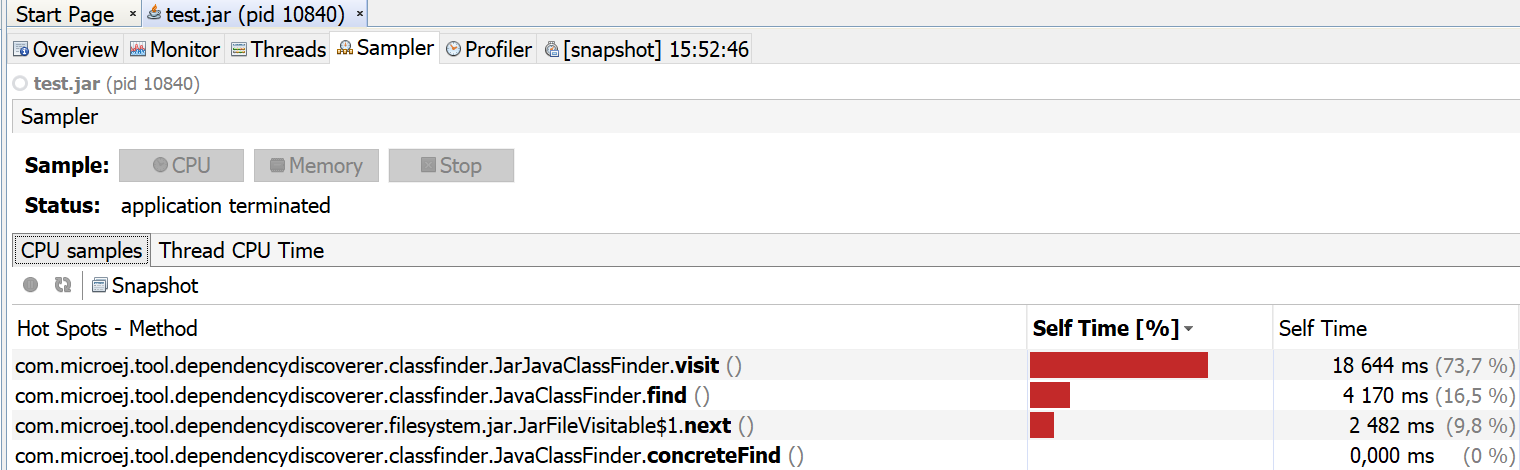
\includegraphics[width=\textwidth]{./ressources/images/timeRepartitionByMethodssheer.png}
\end{center}

73,7 \% du temps d’exécution est passé dans la méthode visit() de la classe JarJavaClassFinder. Il se trouve que cette fonction est dédiée à la lecture des fichiers jars à analyser.La méthode va ouvrir les jars puis itérer au travers de leur contenu en appelant la méthode next(), présente sur le graphique et représentant 9,8 \% du temps d’exécution. Cette routine est appelée par la méthode find() , 16,5 \% du temps d’exécution. En cumulant le temps passé dans la méthode find() et toute les méthodes qu'elle appelle, on arrive à 100 \% du temps d’exécution à 10-1 près. La question est donc : à quoi sert cette fonction et s'il est normale qu’elle soit si lente?

Lorsqu’une classe est référencée dans du code analysé, celle-ci est récupérée. Soit pour trouver d’autres dépendances par analyse récursive soit pour la rajouter directement comme dépendance. Si elle est déjà chargée en tant que nœud ASM elle est récupérée en local, sinon la méthode find() est appelée. Celle ci va alors parcourir et ouvrir tous les fichiers jar du againstClasspath jusqu’à trouver la classe.

Pour ce qui est de la justification du temps de traitement, il est de notoriété commune que les I/O et en particulier les I/O sur disque sont à éviter car très lentes. Il est aussi évident que parcourir l’entièreté des fichiers jar du dépôt MicroEJ revient à plusieurs centaines d’ouvertures de fichiers jar et plusieurs milliers d’opérations de lecture. Dans ces conditions il est donc ‘normale’ que la méthode de recherche soit si lente.

En résumé, le seul moyen d’optimiser la recherche dans les jars était de ne pas rechercher dans les jars; la possibilité la plus simple étant de charger et analyser tous les jars au lancement du programme. Cette ‘solution’ implique cependant un temps de traitement irréductible pour toute recherche et une consommation mémoire conséquente. Heureusement il se trouve qu’un problème similaire avait déjà été rencontré dans un autre programme MicroEJ. La solution est d'utiliser une variable cache qui enregistrait la liste des entées de chaque jars. La variable est donc assez légère car elle ne contient qu’une liste de noms. Le nombre d’I/O est cependant beaucoup plus faible car une fois tous les jars chargés 1 fois il est possible de savoir exactement ou se trouve chaque classe. Récupérer une classe ne nécessitera donc plus qu’une seule ouverture et une seule lecture de jar.

\subsection{Résultats de l’optimisation}

\begin{center}
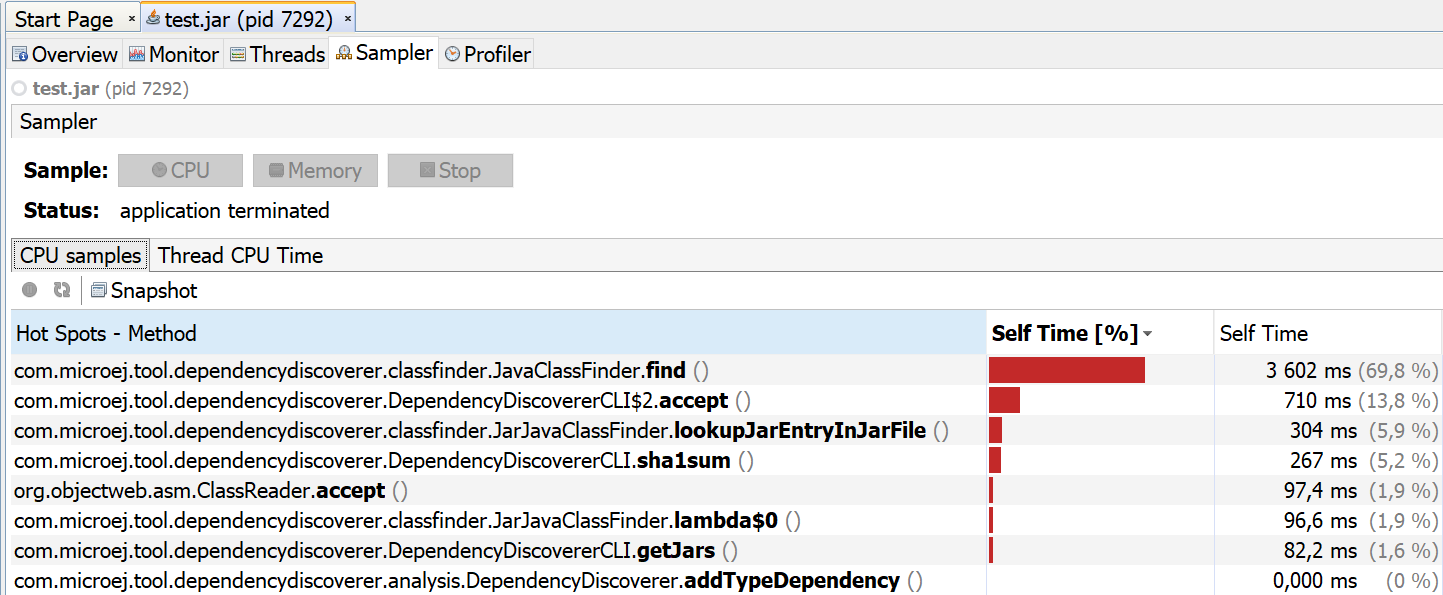
\includegraphics[width=\textwidth]{./ressources/images/timeRepartitionByMethodsCachedsheer.png}
\end{center}

Comme attendu, les résultats après avoir implémenté ce système sont bien meilleurs.
La majorité du temps est toujours passée dans la lecture de jars mais la durée globale n’est plus que de 5 secondes. De plus, avec le cache, l’augmentation sera beaucoup plus faible car, même si le dépôt MicroEJ doublait de taille, après mise en cache, il n’y aurait toujours qu’une opération d’ouverture et de lecture de jar pour chercher une classe. On peut donc s’attendre à ce que le programme reste sous la minute d’exécution dans la plupart des cas. Le temps d’exécution est donc convenable.

Ce problème a cependant montré qu'un aspect avait été négligé. Le programme gère bien les logs d’erreurs, mais aucune information n’est renvoyée pendant l’exécution, ce qui peut paraître anormal au delà de 10 secondes sans retours. Ajouter un indicateur de l’avancement pourrait donc être souhaitable afin d’éviter aux utilisateurs d’attendre sans indication sur l’état du programme.


\chapter{Etranger}
%Si les échanges avec d'autres pays sont simple sur internet, il est souvent nécessaire de connaître la langue et la culture d'un pays lorsqu'on veut se rendre sur place pour des études ou le travail

Les prérequis du diplôme d'ingénieurs comprennent une mobilité à l'international, celle-ci peut consister en un stage ou un semestre d'étude. Cela permet de gagner en autonomie à travers une meilleure ouverture d'esprit sur les différentes façons de vivre et travailler. Apportant un recul nécessaire au travail dans un contexte mondialisé. 


Pour ma mobilité je devais réaliser un semestre d'étude au Japon, dans l'université de Hyogo. La pandémie m’en a empêché mais j’avais cependant effectué toutes les procédures d’inscription et même trouvé un logement. Le japonais est un langage extrêmement éloigné des langues européennes , le système d’écriture et la structure des phrases sont différents. L’anglais est donc très difficile à apprendre pour les japonais et inversement apprendre le japonais est très complexe pour un européen.% De ce fait j'ai pris de l'avance en passant mon toeic en avance et ai pris des cours 
Mon contact sur place était un enseignant-chercheur japonais dont le niveau d’anglais était suffisant pour que nous puissions communiquer, il m’a aidé pour les démarches administratives qui devait être réalisé sur place. J’ai cependant rencontré des difficultés car la plupart des ressources écrites étaient rédigées exclusivement en japonais. J’ai par exemple dû traduire la liste de cours que j’avais choisit de suivre pour que Polytech puisse les valider .

Un séjour d'études au japon présente quelques difficultés mais reste envisageable sans une connaissance profonde du pays. Cela est différent si l'on a pour objectif de s'y installer.
Les codes du monde du travail Japonais sont très stricts, le respect des supérieurs est absolue, il faut d'ailleurs utiliser une variation honorifique du langage que les natifs eux-même peinent à maîtriser .
Contrairement à la France très peu d'étrangers vivent au Japon. Toutes les personnes vivant là-bas rapportent que même après des dizains d’années et une maîtrise de la langue et de la culture ils restent des étranger et subissent une certaine exclusion.\\

Même si il y a beaucoup plus d'étrangers en France ils rencontrent aussi des difficultés. Durant ma formation j'ai rencontrer étudiants de différentes nationalités qui faisaient fasse à ces difficultés. L'un était réfugié Syrien et a du reprendre des études d'ingénieurs car son diplôme n'était pas reconnu en France. Il a dû apprendre le français seul et suivre le cursus sans aménagements.
Un autre n'avais pas encore effectué la démarche de naturalisation Française pour ne pas perdre sa nationalité Mongole, rendant plus compliqué un retour en Mongolie pour voir sa famille. Il devait par conséquent renouveler un visa tout les ans ce qui imposait qu'il possède un minimum d'argent d'avance, il a donc du travailler une partie de ces études pour respecté cette contrainte.
Les avoir rencontré m'a permit de me rendre compte de l'isolement et des difficultés rencontrés en France.\\

Grâce à internet, l’informatique évolue mondialement car toute les ressources sont disponible partout dans le monde. Pour que les échange soit possible entre tous les pays  l’anglais s’est imposé comme langue commune. Cela s’explique par le grand nombre d’utilisateur de l’anglais mais je pense surtout sur la simplicité de la langue à l’écrit, pour l’informatique la plupart des langages sont basés sur l’anglais il y a donc une raison en plus de l’utiliser.
Les outils informatiques aussi sont communs pour deux raisons principales:
-Les contraintes de développement informatique sont similaires quelque soit le domaine (web, logiciels ...)
-De très bon outils open source maintenus par la communauté ont émergé et se sont imposés dans le monde.
Je pondérerais avec des contre-exemple comme la Chine où le niveau d’anglais est souvent trop bas pour que les échanges fluides. Ou le Japon qui communique souvent sur des sites inconnus hors du japons. 
D’un point de vu général, l’environnement mondial autour de l’IT est pour moi un très bon exemple d’une collaboration international fonctionnelle.\\

En conclusion, s’intégrer dans d'autres pays peut être très compliqué et il est nécessaire de se renseigné avant d'aller travailler à l'étranger. Cela comprend l'apprentissage de la langue mais aussi la culture. Cela peut décourager mais mon expérience m'a montré que partager les cultures permet une meilleurs ouverture d'esprit et de partager des connaissances et compétences ainsi que de mettre au point des projets communautaires à l'influence mondiale.

\chapter{Conclusion}

La formation des nouveaux arrivants m'a permis de prendre en main les différents outils utilisés par l'entreprise en développant une application de mon choix. J'ai appris à utiliser des outils de gestion de projets informatiques tels que Git ou Jenkins, permettant d'appliquer des cycles d'intégration et déploiement continus.
Je me suis aussi familiarisé avec les différents moyens de communication qui permettent de garder des liens entre les employés.\\

J'ai ensuite travaillé sur le Dependency Discoverer. J'ai effectué une refonte comprenant : une mise à jour de sa compatibilité, la possibilité d'une utilisation en ligne de commande et l'ajout d'options pour l’utilisateur. 

Je me suis aussi occupé du passage du code en open source en deux phases. D'abord en modifiant le code pour qu'il respecte les standards de qualité exigés par l'entreprise. Ensuite, en mettant en place un cycle d'intégration complet automatisant les tests et la compilation du code dans un exécutable. 

Ce travail a nécessité de nombreuses recherches pour adapter le cycle de production de l'entreprise à un projet open source nécessitant des outils externes.\\

Pour finir j'ai créé différentes documentations autour du Dependency Discoverer. Celles destinées aux utilisateurs et celles destinées aux développeurs de MicroEJ, constituées de tutoriels compilant le travail de R\&D réalisé.\\

Tout au long de mon stage j’ai appris à utiliser de nouveaux outils d’assistance aux développement informatique, en particulier pour la gestion de projets et le travail collaboratif. J'ai acquis la capacité à créer du code performant et optimisé pour la machine tout en assurant sa lisibilité. J'ai appris à produire un travail suffisamment documenté et propre pour que la maintenance soit assurée par d'autres développeurs.\\

Ce stage clôture mes 5 années de formation à Polytech durant lesquelles j'ai découvert les domaines de l'informatique et de l'électronique. 
Mon expérience au sein de MicroEJ m’a apporté la maîtrise d'outils permettant d'appliquer mes compétences techniques avec une rigueur professionnelle. J'ai appris à créer des produits en visant une utilisation par le grand public.\\ 

Mon expérience chez MicroEJ est une réussite. Tout d'abord, et malgré le travail en distanciel, je me suis senti complètement intégré à l'équipe. Mais surtout parce que le travail que j'ai réalisé va avoir un impact sur la durée pour l'entreprise et ses clients. Enfin, le passage en open source du Dependency Discoverer s'inscrivait dans une démarche de collaboration et de partage que je supporte, ce qui m'a d'autant plus impliqué. J'espère que mes emplois futurs n’amènerons à travailler à nouveau sur ce type de projets.


\chapter*{Bibliographie}
\addcontentsline{toc}{chapter}{Bibliographie}

\subsubsection{Page Github du Dependency Discoverer}

\href{https://github.com/MicroEJ/Tool-ApiDependencyDiscoverer}{https://github.com/MicroEJ/Tool-ApiDependencyDiscoverer}

\subsubsection{Page Github de MicroEJ contenant tous les projets publics dont le Dependency Discoverer}

\href{https://github.com/MicroEJ}{https://github.com/MicroEJ}

\subsubsection{Source principale d'exemples et conseils : stack overflow}

\href{https://stackoverflow.com/}{https://stackoverflow.com/}

\subsubsection{Documentation officielle d'ASM}

\href{https://asm.ow2.io/}{https://asm.ow2.io/}

\subsubsection{Documentation officielle de picocli}

\href{https://picocli.info}{https://picocli.info}

\subsubsection{Documentation officielle de GraalVM}

\href{https://www.graalvm.org/}{https://www.graalvm.org/}

\subsubsection{Documentation officielle de TravisCI}

\href{https://docs.travis-ci.com/}{https://docs.travis-ci.com/}

\subsubsection{Documentation officielle de Github action}

\href{https://docs.github.com/en/actions}{https://docs.github.com/en/actions}

\subsubsection{Site officiel d'openweathermap, contient les documentations utilisées pendant le stage}

\href{https://openweathermap.org/}{https://openweathermap.org/}

\subsubsection{Documentation officielle de VisualVM}

\href{https://visualvm.github.io/}{https://visualvm.github.io/}

\subsubsection{Site principal de MicroEJ}

\href{https://www.microej.com/}{https://www.microej.com/}

\subsubsection{Documentation publique de MicroEJ}

\href{https://docs.microej.com/en/latest/}{https://docs.microej.com/en/latest/}

\subsubsection{Site développeur de MicroEJ}

\href{https://developer.microej.com/}{https://developer.microej.com/} 

\subsubsection{Site officiel de RocketChat}

\href{https://rocket.chat/}{https://rocket.chat/}

\subsubsection{Site officiel Ant, contient aussi les documentations}

\href{https://ant.apache.org/}{https://ant.apache.org/}

\subsubsection{Site officiel d'Ivy}

\href{https://ant.apache.org/ivy/}{https://ant.apache.org/ivy/}

\subsubsection{Site officiel de Jfrog}

\href{https://www.jfrog.com/}{https://www.jfrog.com/}

\subsubsection{Site officiel de Jenkins}

\href{https://www.jenkins.io/}{https://www.jenkins.io/}

\subsubsection{Site officiel de Youtrack}

\href{https://www.jetbrains.com/youtrack/}{https://www.jetbrains.com/youtrack/}

\subsubsection{Site officiel de Git}

\href{https://git-scm.com/}{https://git-scm.com/}

\subsubsection{Dépôt central MicroEJ}

\href{https://docs.microej.com/en/latest/overview/repository.html\#central-repository}{https://docs.microej.com/en/latest/overview/repository.html\#central-repository}

\subsubsection{Modele Git utilisé par l'entreprise}

\href{https://nvie.com/posts/a-successful-git-branching-model/}{https://nvie.com/posts/a-successful-git-branching-model/}

\begin{appendices}
    
\chapter*{Codes}
\addcontentsline{toc}{chapter}{Codes}

\section*{Retour javap -v testASM.class}
\addcontentsline{toc}{section}{\protect\numberline{}Retour javap -v testASM.class}
\label{javapVtestASM}

\begin{lstlisting}
public class TestASM
  minor version: 0
  major version: 55
  flags: (0x0021) ACC_PUBLIC, ACC_SUPER
  this_class: #3                          // TestASM
  super_class: #4                         // java/lang/Object
  interfaces: 0, fields: 0, methods: 2, attributes: 1
Constant pool:
   #1 = Methodref          #4.#13         // java/lang/Object."<init>":()V
   #2 = String             #14            // this is a test
   #3 = Class              #15            // TestASM
   #4 = Class              #16            // java/lang/Object
   #5 = Utf8               <init>
   #6 = Utf8               ()V
   #7 = Utf8               Code
   #8 = Utf8               LineNumberTable
   #9 = Utf8               testStringDependency
  #10 = Utf8               ()Ljava/lang/String;
  #11 = Utf8               SourceFile
  #12 = Utf8               TestASM.java
  #13 = NameAndType        #5:#6          // "<init>":()V
  #14 = Utf8               this is a test
  #15 = Utf8               TestASM
  #16 = Utf8               java/lang/Object
{
  public TestASM();
    descriptor: ()V
    flags: (0x0001) ACC_PUBLIC
    Code:
      stack=1, locals=1, args_size=1
         0: aload_0
         1: invokespecial #1                  // Method java/lang/Object."<init>":()V
         4: return
      LineNumberTable:
        line 2: 0

  public java.lang.String testStringDependency();
    descriptor: ()Ljava/lang/String;
    flags: (0x0001) ACC_PUBLIC
    Code:
      stack=1, locals=1, args_size=1
         0: ldc           #2                  // String this is a test
         2: areturn
      LineNumberTable:
        line 5: 0
}
\end{lstlisting}
 
\section*{Fichier build ant}
\addcontentsline{toc}{section}{\protect\numberline{}Fichier build ant}
\label{antBuild}
\lstinputlisting{ressources/code/build.xml}
    
\chapter*{Images}
\addcontentsline{toc}{chapter}{Images}

\section*{ClassNode}

Affichage du contenu d'une variable ClassNode avec l'outil d'Eclipse. Seules les lignes surlignées contiennent des informations à analyser. Toute la hiérarchie n'est pas visible.

\addcontentsline{toc}{section}{\protect\numberline{}ClassNode}
\label{ClassNode}

\begin{center}
 	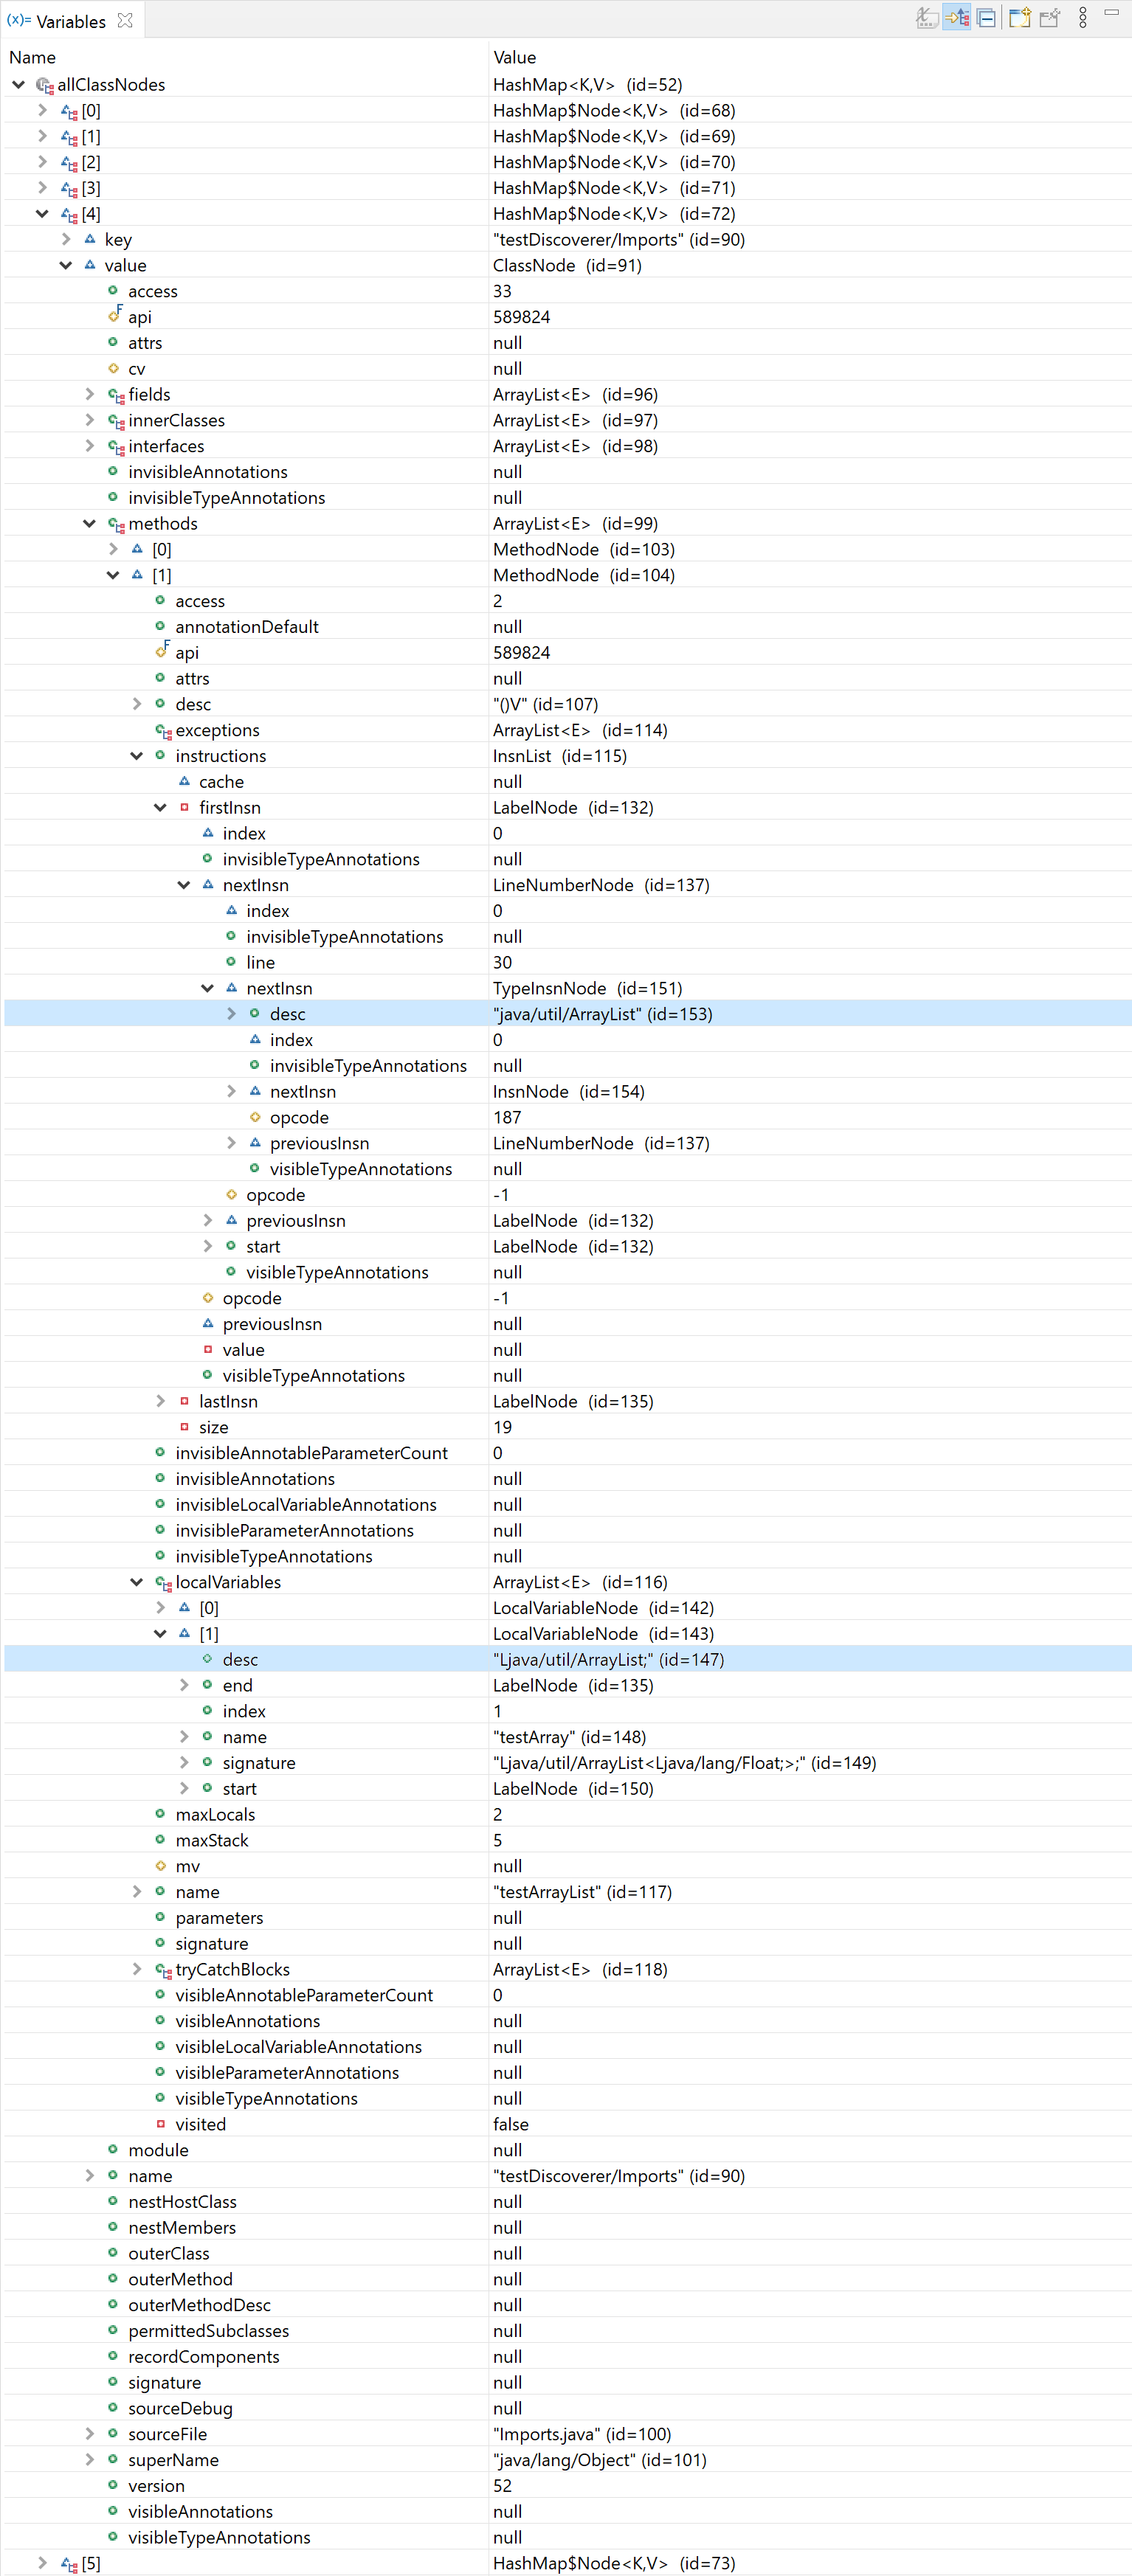
\includegraphics[trim=0in 10.01in 0in 0in, clip, width =\textwidth]{ressources/images/ClassNode.png}

	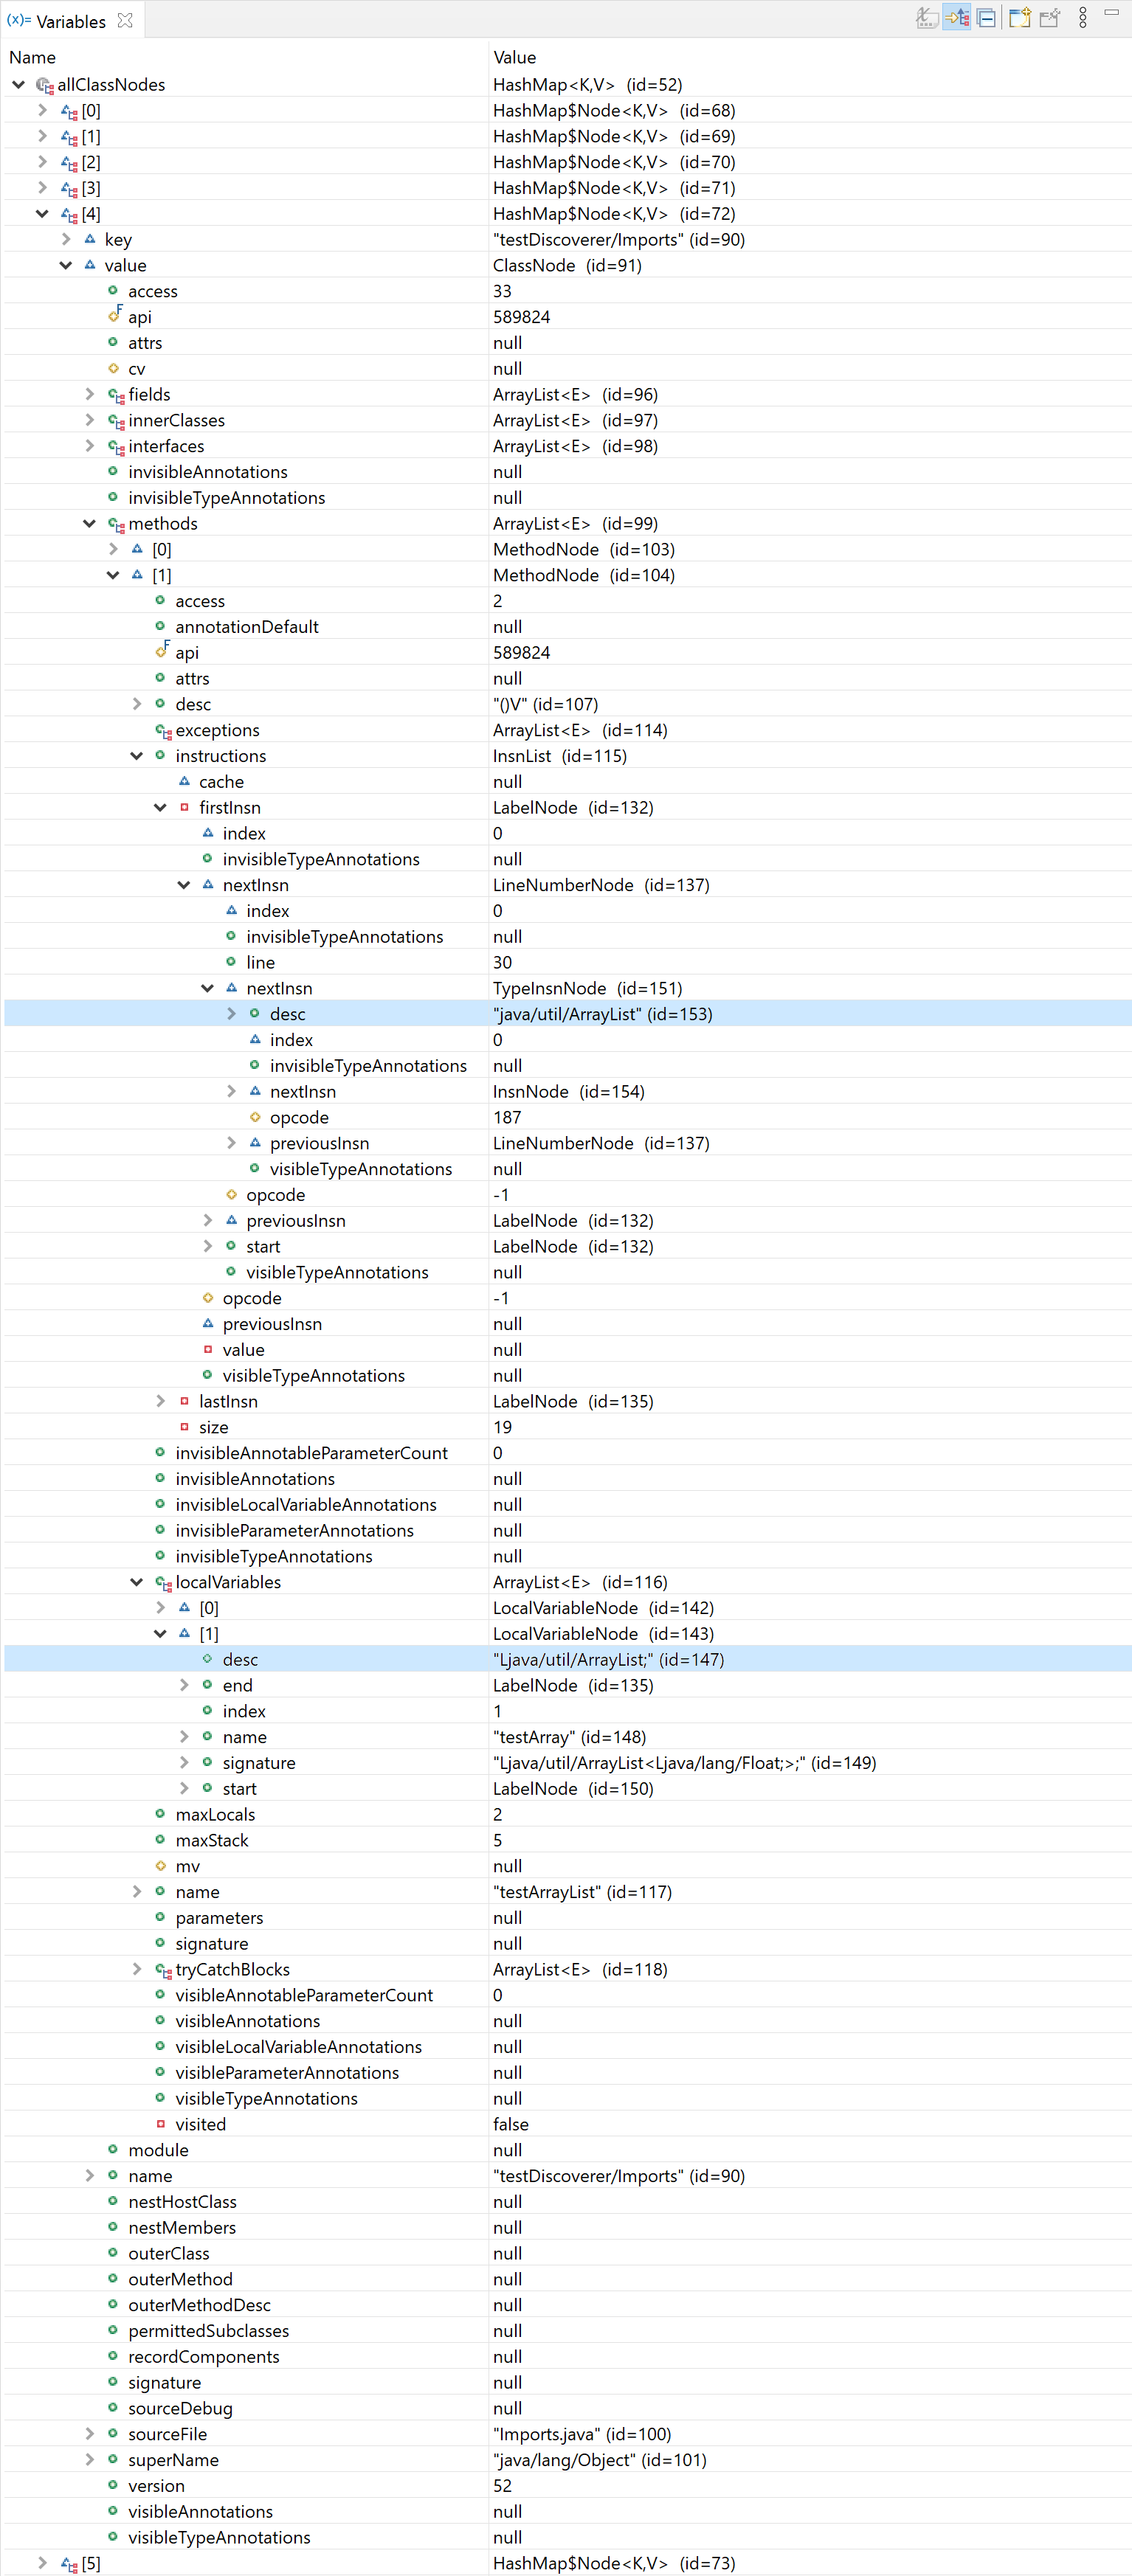
\includegraphics[trim=0in 0in 0in 8.18in, clip,width =\textwidth]{ressources/images/ClassNode.png}

\end{center}



\chapter*{Compétences}
\addcontentsline{toc}{chapter}{Compétences}
\label{competences}
\newcolumntype{b}{>{\hsize=1.8\hsize}X}
\newcolumntype{s}{>{\hsize=.2\hsize}X}

\definecolor{darkBluePolytech}{HTML}{366092}
\definecolor{darkerBluePolytech}{HTML}{1f497d}
\color{darkerBluePolytech}

\def\arraystretch{1.5}

\noindent
\begin{tabularx}{\textwidth}{ | s | b | } 
 \rowcolor{darkBluePolytech}
 \multicolumn{2}{|>{\hsize=\dimexpr2\hsize+2\tabcolsep+\arrayrulewidth\relax}X|}{\textcolor{white}{TC1 - Gérer et conduire un projet de sa conception à sa réalisation selon ses dimensions techniques, économiques et humaines}}\\
  
 \hline\hline
	\hypertarget{TC11}{TC1.1.} & en maîtrisant les bases du management opérationnel\\
 \hline
\hypertarget{TC12}{TC1.2.} & en étant apte à choisir et/ou mettre en œuvre des outils et des méthodes pour la réalisation du projet\\
\hline
\hypertarget{TC13}{TC1.3.} & en étant apte à mobiliser les ressources d'un champ scientifique et technique spécifique\\
\hline
\hypertarget{TC14}{TC1.4.} & en intégrant les aspects économiques et financiers du projet\\
\hline
\hypertarget{TC12}{TC1.5.} & en étant apte à évoluer dans un contexte de collaboration multi-acteurs\\
\hline
\end{tabularx}

\noindent
\begin{tabularx}{\textwidth}{ | s | b | } 
\hline
\rowcolor{darkBluePolytech}
\multicolumn{2}{|>{\hsize=\dimexpr2\hsize+2\tabcolsep+\arrayrulewidth\relax}X|}{\textcolor{white}{TC2 - Communiquer efficacement avec un public varié, et développer son projet professionnel}}\\
\hline\hline
 \hypertarget{TC21}{TC2.1.} & en s'appropriant les clés d'une communication adaptée : 1. transmettre un message oral\\	
\hline
 \hypertarget{TC22}{TC2.2.} & en s'appropriant les clés d'une communication adaptée : 2. rédiger un écrit professionnel\\
\hline
 \hypertarget{TC23}{TC2.3.} & en opérant des choix professionnels et en mettant en place une stratégie adaptée pour atteindre ses objectifs et en développant une attitude assertive\\
\hline
 \hypertarget{TC24}{TC2.4.} & en évaluant et faisant évoluer ses compétences dans une dynamique apprenante\\
\hline
\end{tabularx}

\noindent
\begin{tabularx}{\textwidth}{ | s | b | } 
\hline
 \rowcolor{darkBluePolytech}
\multicolumn{2}{|>{\hsize=\dimexpr2\hsize+2\tabcolsep+\arrayrulewidth\relax}X|}{\textcolor{white}{TC3 - Mobiliser et développer les compétences en sciences humaines nécessaires à son intégration et au développement de son entreprise et de la société}}\\
\hline\hline
 \hypertarget{TC14}{TC3.1.} & en s'intégrant dans l'entreprise et en exerçant le métier d'ingénieur\\	
\hline
\hypertarget{TC32}{TC3.2.} & en prenant en compte les enjeux industriels, économiques et professionnels\\
\hline
\hypertarget{TC33}{TC3.3.} & en travaillant en contexte pluriculturel et/ou international\\
\hline
\hypertarget{TC34}{TC3.4.} & en étant apte à prendre en compte les enjeux et les besoins de la société\\	
\hline
\end{tabularx}
 
\noindent
\begin{tabularx}{\textwidth}{ | s | b | } 
\hline
 \rowcolor{darkBluePolytech}
\multicolumn{2}{|>{\hsize=\dimexpr2\hsize+2\tabcolsep+\arrayrulewidth\relax}X|}{\textcolor{white}{TC4 - Développer des activités contribuant à des innovations ou des avancées scientifiques}}\\
\hline\hline
\hypertarget{TC41}{TC4.1.} & en situant son activité par rapport à l'état de l'art des connaissances et/ou des pratiques\\
\hline
\hypertarget{TC42}{TC4.2.} & en menant un travail de recherche fondamentale ou appliquée cohérent avec une analyse critique des résultats\\
\hline
\hypertarget{TC43}{TC4.3.} & en développant une démarche créative s'inscrivant dans un contexte d'innovation\\
\hline
\hypertarget{TC44}{TC4.4.} & en s'appuyant sur des techniques de management de l'innovation dans une démarche d'ouverture et d'entreprenariat\\
\hline
\end{tabularx}

\end{appendices}
   
\end{document}
